%% ============================================================
%%  IntelliCode Review — Master's Thesis
%%  Safaa Patel, University of Nevada, Reno
%%  Template adapted from UNR Graduate School guidelines
%% ============================================================

\documentclass[12pt, oneside]{report}

%% ---- Packages ----
\usepackage[margin=1in]{geometry}
\usepackage{setspace}
\usepackage{times}
\usepackage{amsmath, amssymb}
\usepackage{graphicx}
\usepackage{xcolor}
\usepackage{listings}
\usepackage{booktabs}
\usepackage{longtable}
\usepackage{array}
\usepackage{multirow}
\usepackage{hyperref}
\usepackage{acronym}
\usepackage{caption}
\usepackage{subcaption}
\usepackage{float}
\usepackage{enumitem}
\usepackage{fancyhdr}
\usepackage{tocloft}
\usepackage{titlesec}
\usepackage{microtype}
\usepackage{cite}
\usepackage{url}
\usepackage{rotating}
\usepackage{tikz}
\usetikzlibrary{calc, backgrounds}

%% ---- Hyperref Setup ----
\hypersetup{
    colorlinks=true,
    linkcolor=blue,
    citecolor=blue,
    urlcolor=blue,
    pdftitle={IntelliCode Review: An AI-Powered Platform for Automated Code Quality Analysis},
    pdfauthor={Safaa Patel},
}

%% ---- Code Listing Style ----
\definecolor{codebg}{rgb}{0.95,0.95,0.95}
\definecolor{codestr}{rgb}{0.63,0.13,0.94}
\definecolor{codecomment}{rgb}{0.25,0.5,0.35}
\definecolor{codekw}{rgb}{0.0,0.0,0.9}

\lstdefinestyle{pythonstyle}{
    language=Python,
    backgroundcolor=\color{codebg},
    basicstyle=\ttfamily\small,
    keywordstyle=\color{codekw}\bfseries,
    stringstyle=\color{codestr},
    commentstyle=\color{codecomment}\itshape,
    numberstyle=\tiny\color{gray},
    numbers=left,
    numbersep=5pt,
    breaklines=true,
    showstringspaces=false,
    frame=single,
    captionpos=b,
}

\lstdefinestyle{jsstyle}{
    language=JavaScript,
    backgroundcolor=\color{codebg},
    basicstyle=\ttfamily\small,
    keywordstyle=\color{codekw}\bfseries,
    stringstyle=\color{codestr},
    commentstyle=\color{codecomment}\itshape,
    numbers=left,
    numbersep=5pt,
    breaklines=true,
    showstringspaces=false,
    frame=single,
    captionpos=b,
}

\lstset{style=pythonstyle}

%% ---- Spacing ----
\doublespacing

%% ---- Header/Footer ----
\pagestyle{fancy}
\fancyhf{}
\rhead{\thepage}
\lhead{\leftmark}
\renewcommand{\headrulewidth}{0.4pt}

%% ---- Chapter Title Format ----
\titleformat{\chapter}[display]
  {\normalfont\Large\bfseries}{\chaptertitlename\ \thechapter}{20pt}{\Huge}

%% ============================================================
\begin{document}

%% ---- Title Page ----
\begin{titlepage}
\begin{center}
\vspace*{1in}
{\Large University of Nevada, Reno}\\[0.5em]
\vspace{1in}
{\LARGE\bfseries IntelliCode Review: An AI-Powered Platform for\\[0.3em]
Automated Code Quality Analysis}\\[1.5in]
{\large A thesis submitted in partial fulfillment of the\\
requirements for the degree of Master of Science\\
in Computer Science and Engineering}\\[1in]
{\large by}\\[0.5em]
{\Large Safaa Patel}\\[1in]
{\large Dr. [Advisor Name], Advisor}\\[1.5in]
{\large May, 2026}
\end{center}
\end{titlepage}

%% ---- Copyright Page ----
\newpage
\thispagestyle{empty}
\vspace*{\fill}
\begin{center}
\textcopyright\ by Safaa Patel\\
All Rights Reserved
\end{center}
\vspace*{\fill}

%% ---- Approval Page ----
\newpage
\thispagestyle{empty}
\begin{center}
{\large THE GRADUATE SCHOOL}\\[1em]
We recommend that the thesis\\
prepared under our supervision by\\[1em]
{\large Safaa Patel}\\[1em]
entitled\\[1em]
{\large\bfseries IntelliCode Review: An AI-Powered Platform for\\
Automated Code Quality Analysis}\\[1em]
be accepted in partial fulfillment of the\\
requirements for the degree of\\[1em]
{\large MASTER OF SCIENCE}\\[2em]
Dr. [Advisor Name], Advisor\\[1.5em]
Dr. [Committee Member 1], Graduate School Representative\\[1.5em]
Markus Kemmelmeier, Ph.D., Dean,\\
Graduate School\\[1.5em]
May, 2026
\end{center}

%% ---- Front Matter Numbering ----
\pagenumbering{roman}
\setcounter{page}{1}

%% ============================================================
%%  ABSTRACT
%% ============================================================
\chapter*{Abstract}
\addcontentsline{toc}{chapter}{Abstract}

This thesis makes two connected contributions. The first is \textit{IntelliCode Review},
a web-based platform that integrates twelve analysis components---four trained ML models
and eight deterministic AST-based modules---into a unified code quality system. The second,
and the more technically novel, is a rigorous multi-protocol evaluation that exposes how
badly standard ML evaluation practice overstates performance for code analysis tasks.

It accepts Python source code and reports on security vulnerabilities, cyclomatic and
cognitive complexity, bug probability, code clones, refactoring opportunities, dead code,
technical debt, documentation quality, performance hotspots, dependency coupling, and
readability.

The stack is three-tier: a React~18 SPA (shadcn/ui) on the frontend, a Python FastAPI
backend with twelve specialized REST endpoints, and models built on XGBoost, scikit-learn,
and PyTorch. All reported metrics are post-audit, after correcting a target leakage error
that had artificially inflated complexity figures. The XGBoost complexity predictor achieves
$R^2 = 0.712$ (RMSE = 49.5, Spearman $\rho = 0.865$), with multi-seed
$R^2 = 0.685 \pm 0.044$ across five seeds and LOPO $\rho = 0.795 \pm 0.186$ across ten
repositories. The security Random Forest reaches AUC $= 0.834 \pm 0.036$ in-distribution
but AUC $= 0.494 \pm 0.189$ under LOPO.

The near-chance LOPO result is not a simple generalisation failure. Ablation shows that
removing API co-occurrence features \emph{improves} cross-project AUC---we define this
as \textbf{anti-learning}: \emph{feature--label correlations that invert across training
and test distributions, causing systematically wrong predictions under shift}. This led
to a security feature redesign around a 16-dimensional causal taint-flow representation.
The bug predictor reaches multi-seed AUC $= 0.676 \pm 0.038$ under random split but
drops to walk-forward temporal CV mean AUC $= 0.544 \pm 0.105$
($\Delta\text{AUC} = -0.132$), confirming that random-split defect prediction baselines
are upward-biased. Per-file static metrics cannot, by construction, distinguish a
recently-fixed file from one about to fail; a credible JIT predictor would need sequential
or developer-aware features such as commit history embeddings or temporal graph neural
networks. The pattern classifier reaches cross-validated F1 $= 0.657$ after removing 14
metric features that encode the label rules directly---a confirmed $+0.082$ F1 inflation
from circular label supervision (Wilcoxon $p = 0.031$) in the prior 26-feature model.
All four models were trained from scratch on real OSS datasets. The remaining eight modules
are deterministic and AST-based.

Evaluation covers 24 end-to-end API test cases and a prototype demonstration. Full analysis
completes in under 2\,s; the \texttt{/analyze/quick} endpoint runs in under 500\,ms.

%% ============================================================
%%  DEDICATION
%% ============================================================
\chapter*{Dedication}
\addcontentsline{toc}{chapter}{Dedication}

I dedicate this thesis to my family, whose constant encouragement and sacrifices made my
graduate studies possible. Your belief in me has been my greatest source of strength.

%% ============================================================
%%  ACKNOWLEDGMENTS
%% ============================================================
\chapter*{Acknowledgments}
\addcontentsline{toc}{chapter}{Acknowledgments}

I would like to express my sincere gratitude to my advisor for their guidance, patience, and
intellectual support throughout this work. Their feedback shaped both the research direction
and the quality of this thesis.

I am grateful to the University of Nevada, Reno Department of Computer Science and
Engineering for providing the academic environment and resources that made this project
possible.

I also thank the open-source communities behind Python, FastAPI, React, Vite, XGBoost,
scikit-learn, and PyTorch, whose libraries formed the technical foundation of IntelliCode
Review, and the maintainers of Django, Flask, requests, and pip whose public repositories
provided the real training data used in this work.

Finally, I thank my family and friends for their unwavering support throughout my graduate
studies. Without their encouragement, this work would not have been possible.

%% ============================================================
%%  TABLE OF CONTENTS / FIGURES / TABLES
%% ============================================================
\tableofcontents
\listoftables
\listoffigures

%% ---- List of Acronyms ----
\chapter*{List of Acronyms}
\addcontentsline{toc}{chapter}{List of Acronyms}

\begin{acronym}[SQALE]
  \acro{AI}{Artificial Intelligence}
  \acro{API}{Application Programming Interface}
  \acro{AST}{Abstract Syntax Tree}
  \acro{AUC}{Area Under the ROC Curve}
  \acro{CI}{Continuous Integration}
  \acro{CNN}{Convolutional Neural Network}
  \acro{CORS}{Cross-Origin Resource Sharing}
  \acro{CSS}{Cascading Style Sheets}
  \acro{CWE}{Common Weakness Enumeration}
  \acro{HTML}{Hypertext Markup Language}
  \acro{HTTP}{Hypertext Transfer Protocol}
  \acro{JSON}{JavaScript Object Notation}
  \acro{LR}{Logistic Regression}
  \acro{MI}{Maintainability Index}
  \acro{ML}{Machine Learning}
  \acro{MLP}{Multilayer Perceptron}
  \acro{NLP}{Natural Language Processing}
  \acro{PR}{Pull Request}
  \acro{REST}{Representational State Transfer}
  \acro{RF}{Random Forest}
  \acro{ROC}{Receiver Operating Characteristic}
  \acro{RMSE}{Root Mean Squared Error}
  \acro{SPA}{Single-Page Application}
  \acro{SQALE}{Software Quality Assessment based on Lifecycle Expectations}
  \acro{SAST}{Static Application Security Testing}
  \acro{SSE}{Server-Sent Events}
  \acro{SQL}{Structured Query Language}
  \acro{TF-IDF}{Term Frequency--Inverse Document Frequency}
  \acro{UI}{User Interface}
  \acro{UX}{User Experience}
  \acro{XSS}{Cross-Site Scripting}
\end{acronym}

%% ============================================================
%%  MAIN CONTENT
%% ============================================================
\pagenumbering{arabic}
\setcounter{page}{1}

%% ============================================================
\chapter{Introduction}
\label{ch:intro}
%% ============================================================

\section{Problem Statement}
\label{sec:problem}

Software quality assurance is a multifaceted challenge that pervades every stage of
the software development lifecycle. Despite decades of research in program analysis,
formal verification, and automated testing, code quality defects remain costly: the
National Institute of Standards and Technology (NIST) estimated that software bugs
cost the US economy approximately \$60 billion annually~\cite{nist2002}. Poor code
quality manifests in many forms: security vulnerabilities that expose user data, high
cyclomatic complexity that increases bug density, untested code paths, duplicated logic,
and mounting technical debt that slows future development.

Traditional code review---where a human peer reads and comments on code changes---is
the industry-standard quality gate. However, manual review has well-documented
limitations. Reviewers are inconsistent: the same code may be evaluated differently by
different engineers, or even by the same engineer at different times~\cite{bacchelli2013}.
Review quality degrades under time pressure~\cite{mcintosh2016}. Reviewers are better
at detecting style violations than logical bugs~\cite{fagan1976}. And as teams scale
and codebases grow, the ratio of reviewers to code changes worsens.

Static analysis tools address some of these limitations by automating rule-based
checks. Tools such as Pylint, Flake8, and Bandit scan Python code for style violations,
syntax errors, and known vulnerability patterns. However, they are limited to
pattern-matching against a fixed rule set; they do not learn from project history,
cannot predict \textit{future} bugs, and do not produce a holistic quality score
that integrates multiple dimensions of code health into a single actionable report.

\section{Proposed Solution}
\label{sec:solution}

This thesis proposes and implements \textit{IntelliCode Review}, an AI-powered web
platform that unifies twelve complementary analysis models into a single, developer-friendly
interface. The system's key contributions are:

\begin{enumerate}[label=\arabic*.]
  \item A \textbf{twelve-model ML ensemble} covering security, complexity, bugs, patterns,
    clone detection, refactoring, dead code, technical debt, documentation quality,
    performance, dependency coupling, and readability.
  \item A \textbf{FastAPI backend} that exposes each model as an independent REST endpoint
    and a combined \texttt{/analyze} endpoint that runs all models in a single request.
  \item A \textbf{React 18 frontend} with a rich dashboard, per-review detail pages,
    analytics, and persistent history stored in browser localStorage.
  \item A \textbf{training pipeline} that fetches and processes real labeled data from
    open-source repositories and CVE databases, and trains four ML models end-to-end
    with checkpoints reproducible by running \texttt{train\_all.py}.
  \item A \textbf{reproducible prototype} validated through functional testing and a
    structured evaluation against real Python code samples.
\end{enumerate}

\section{Research Questions}
\label{sec:rq}

This thesis addresses the following research questions:

\begin{description}
  \item[RQ1] Can a unified ML-based platform provide more comprehensive and actionable
    code quality feedback than traditional single-purpose static analysis tools?
  \item[RQ2] What machine learning architectures are most appropriate for each of the
    twelve code quality analysis tasks, and how do they perform when trained on real
    open-source code data?
  \item[RQ3] How can a web-based code review platform be designed to be responsive,
    persistent, and practical for real-world developer workflows?
\end{description}

\section{Scope and Limitations}
\label{sec:scope}

IntelliCode Review performs deep ML-based analysis for Python source code and
rule-based security and complexity analysis for JavaScript, TypeScript, and Java via a
tree-sitter multi-language adapter. The repository scanner recognises sixteen programming
languages (Python, JavaScript, TypeScript, Java, C, C++, Go, Rust, Ruby, PHP, Swift,
Kotlin, Scala, R, Dart, and Shell) for file-level metrics. For JavaScript, TypeScript,
and Java submissions, the security scanner applies language-specific regex rule sets
(covering XSS, SQL injection, command injection, weak cryptography, and other CWE-mapped
patterns), and the complexity analyser uses tree-sitter ASTs to compute cyclomatic and
cognitive complexity with rule-based scoring. The ML-trained models for bug prediction
and pattern recognition operate on Python only. The platform integrates with GitHub for repository scanning: users
can connect a GitHub personal access token to trigger batch scans of entire repositories
from the Repositories page. The API also accepts optional git metadata (code churn, author
count, file age, past bug count, commit frequency) to augment bug prediction.

The trained ML models are trained on real open-source dataset samples (3000 per model)
sourced from Django, Flask, requests, pip, and CVE-annotated commits. Real-world
generalisation to unseen production codebases is inherently limited by the diversity of
training data; users should treat model probabilities as risk indicators rather than
deterministic verdicts.

\section{Thesis Organization}
\label{sec:organization}

The remainder of this thesis is organized as follows. Chapter~\ref{ch:background} provides
background on code review, static analysis, and the ML techniques used. Chapter~\ref{ch:related}
surveys related work in automated code review, defect prediction, and developer tooling.
Chapter~\ref{ch:motivation} describes the motivation for the proposed system and formalizes
the design goals. Chapter~\ref{ch:design} details the software architecture and implementation.
Chapter~\ref{ch:demo} presents a prototype demonstration. Chapter~\ref{ch:eval} presents
the evaluation methodology and results. Chapter~\ref{ch:conclusion} concludes and discusses
future work.

%% ============================================================
\chapter{Background}
\label{ch:background}
%% ============================================================

\section{Code Review in Software Engineering}
\label{sec:bg-codereview}

Code review is the systematic examination of source code by one or more individuals other
than the original author, with the goal of finding defects, improving quality, and
transferring knowledge within a team~\cite{fagan1976}. Formal inspection, introduced by
Fagan~\cite{fagan1976} at IBM in the 1970s, was the precursor to modern lightweight
peer review. Today, the predominant form is \textit{modern code review}~\cite{bacchelli2013},
conducted asynchronously via pull requests on platforms such as GitHub, GitLab, and Gerrit.

Studies of code review in practice reveal that reviewers focus primarily on understandability,
coding conventions, and functional correctness---in that order~\cite{bacchelli2013}. Security
defects and performance issues are relatively rarely caught by reviewers~\cite{mcintosh2016}.
This motivates automated tooling that can reliably surface these harder-to-detect issues.

\subsection{Pull-Request-Based Review}

Modern development teams submit code changes as pull requests (PRs), which are reviewed
by one or more peers before merging into the main branch. PR-based review provides a natural
integration point for automated analysis tools, which can comment on PRs with findings
before human review begins. IntelliCode Review is designed to complement this workflow: a
developer pastes a code snippet or submits a file, receives an automated quality report,
and uses that report to self-review before requesting peer feedback.

\subsection{Cost of Poor Code Quality}

Technical debt---the implied cost of future rework caused by choosing a quick solution
over a better one---accumulates with poor code quality. The SQALE (Software Quality
Assessment based on Lifecycle Expectations) methodology~\cite{letouzey2012} quantifies
technical debt in person-hours required to fix each quality issue category. IntelliCode
Review implements a SQALE-inspired debt estimator that aggregates findings from security,
complexity, clone detection, dead code, and refactoring models into a single debt report.

\section{Static Analysis}
\label{sec:bg-static}

Static analysis examines source code without executing it. It encompasses a broad range
of techniques from simple lexical pattern matching to full dataflow and taint analysis.

\subsection{Lexical and Syntactic Analysis}

The simplest form of static analysis scans source code as text, searching for known
dangerous patterns using regular expressions. Tools such as Bandit for Python use this
approach to flag uses of \texttt{eval()}, hardcoded passwords, and insecure deserialization.
IntelliCode Review's security pattern scanner (\texttt{security\_patterns.py}) implements
a curated set of regular expressions covering SQL injection, command injection, path
traversal, hardcoded secrets, weak cryptography, insecure deserialization, code injection,
and XXE vulnerabilities.

\subsection{Abstract Syntax Tree Analysis}

The \ac{AST} is a structured tree representation of source code that captures its grammatical
structure without irrelevant syntactic details. Python's standard library provides the
\texttt{ast} module, which parses source code into an AST and enables tree-walking
visitors. IntelliCode Review uses AST analysis extensively: the \texttt{ASTExtractor}
class extracts features including function definitions, call sites, import statements,
string literals, class hierarchies, and control flow constructs. Seven of the twelve
models (clone detection, refactoring, dead code, documentation quality, performance,
dependency, and readability) are implemented as AST visitors or pattern matchers.

\subsection{Complexity Metrics}

Several quantitative metrics characterize code complexity:

\begin{description}
  \item[Cyclomatic Complexity (McCabe)~\cite{mccabe1976}] Counts the number of linearly
    independent paths through a program's control flow graph. Formally, $V(G) = E - N + 2P$
    where $E$ is edges, $N$ is nodes, and $P$ is connected components.
  \item[Cognitive Complexity~\cite{campbell2018}] A successor metric that penalizes
    nested control structures more heavily, arguing that nesting is a stronger predictor
    of comprehension difficulty than raw path count.
  \item[Halstead Metrics~\cite{halstead1977}] Derive a family of metrics (volume, difficulty,
    effort, predicted bugs) from counts of operators and operands in the source code.
  \item[Maintainability Index~\cite{oman1992}] A composite metric (0--100 scale) combining
    Halstead volume, cyclomatic complexity, and source lines of code, widely used by
    tools such as Visual Studio.
\end{description}

IntelliCode Review computes all four families of metrics in \texttt{code\_metrics.py} and
uses the resulting 17-dimensional feature vector as input to the XGBoost complexity model.

\section{Machine Learning for Code Analysis}
\label{sec:bg-ml}

\subsection{Defect Prediction}

The application of statistical and machine learning techniques to predict software defects
has a rich research history dating to the early 2000s~\cite{nagappan2005, zimmermann2007}.
Early work used product metrics (lines of code, complexity) and process metrics (code churn,
developer experience) as features for logistic regression and na\"ive Bayes classifiers.
Subsequent work demonstrated that more complex models---random forests~\cite{lessmann2008},
support vector machines, and neural networks---could improve prediction accuracy.

IntelliCode Review's bug predictor follows this tradition, combining static code metrics
with optional git metadata (code churn, author count, file age, past bug count, commit
frequency) in a Logistic Regression + XGBoost ensemble, where the gradient-boosted tree
component benefits from early stopping regularisation (best iteration at epoch 97).

\subsection{Vulnerability Detection}

Security vulnerability detection using machine learning has grown rapidly, driven by
the availability of labeled datasets such as Devign~\cite{zhou2019}, D2A, and CodeXGLUE.
Neural approaches range from simple TF-IDF bag-of-tokens classifiers to graph neural
networks operating on code property graphs~\cite{yamaguchi2014}.

IntelliCode Review uses a practical two-component ensemble: (1) a Random Forest classifier
operating on a 25-dimensional feature vector of AST metrics and security-specific counters,
and (2) a 1D Convolutional Neural Network operating on token ID sequences of length 512.
The ensemble combines both predictions via a weighted average ($w_{RF}=0.55$, $w_{CNN}=0.45$).

\subsection{Code Embeddings and Pre-Trained Models}

The introduction of pre-trained transformer models for code---CodeBERT~\cite{feng2020},
GraphCodeBERT~\cite{guo2021}, and CodeT5~\cite{wang2021}---established new state of the
art on a range of code understanding tasks. These models are pre-trained on large corpora
of code and can be fine-tuned for downstream tasks such as vulnerability detection,
clone detection, code summarization, and defect prediction.

IntelliCode Review evaluated a CodeBERT-based approach for pattern recognition but
ultimately implemented the component as a calibrated Random Forest classifier
(\texttt{pattern\_recognition.py}) operating on a 12-dimensional debiased AST feature
vector (structural features only, excluding the 14 metric features that encode label
rules). This choice avoids the \textasciitilde500\,MB model download and GPU requirements
while providing an honest F1=0.657 on four code pattern categories; leakage analysis
confirms that the full 26-feature set inflates F1 by $+0.082$ via circular label
supervision. Section~\ref{ssec:pattern} details this design.

\subsection{Ensemble Methods}

Ensemble methods combine multiple base learners to reduce variance and improve
generalization. Random forests are a bagging ensemble of decision trees; gradient
boosted trees (XGBoost~\cite{chen2016}) train trees sequentially, each correcting
the errors of the previous. IntelliCode Review uses XGBoost for complexity prediction
because of its strong performance on tabular regression tasks and its resistance to
overfitting. The security and bug prediction models both use two-component ensembles
(RF/CNN and LR/XGBoost respectively) to leverage complementary representations.

\section{Web Application Architecture}
\label{sec:bg-web}

\subsection{REST APIs and FastAPI}

\ac{REST}ful \acp{API} are the standard interface for web services, using HTTP verbs
(GET, POST, PUT, DELETE) to operate on resources identified by URIs. FastAPI is a modern
Python web framework built on Starlette and Pydantic that generates OpenAPI documentation
automatically, validates request and response schemas via Python type annotations, and
supports asynchronous request handling via \texttt{asyncio}. FastAPI's performance
(comparable to Node.js and Go for I/O-bound workloads) and developer ergonomics made it
the natural choice for IntelliCode Review's backend.

\subsection{React Single-Page Applications}

React is a component-based JavaScript library for building user interfaces, developed
and maintained by Meta. In React's component model, UI is a function of state: when
state changes, React efficiently re-renders only the affected subtree via a virtual DOM
diffing algorithm. Vite is a next-generation frontend build tool that provides near-instant
hot module replacement during development and optimized production bundles via Rollup.
shadcn/ui is a collection of accessible, unstyled UI components built on Radix UI
primitives and styled with Tailwind CSS utility classes, providing a consistent design
system without imposing a heavy CSS-in-JS runtime.

\subsection{Browser localStorage}

The Web Storage API provides \texttt{localStorage}, a key-value store persisted across
browser sessions with up to 5--10\,MB of capacity per origin. IntelliCode Review uses
localStorage to persist analysis history, user-defined quality rules, and repository
configurations, eliminating the need for a database in the prototype. This approach is
appropriate for a single-user development tool; a production deployment serving multiple
users would require a server-side database.

\section{Technology Stack Summary}
\label{sec:bg-techstack}

Table~\ref{tab:techstack} summarizes the technologies used in IntelliCode Review, all of
which are open-source and freely available.

\begin{table}[H]
\centering
\caption{IntelliCode Review Technology Stack}
\label{tab:techstack}
\begin{tabular}{@{}lll@{}}
\toprule
\textbf{Layer} & \textbf{Technology} & \textbf{Role} \\
\midrule
Frontend framework    & React 18            & Component-based UI \\
Build tool            & Vite 5              & Dev server, HMR, bundling \\
UI components         & shadcn/ui + Radix UI & Accessible component library \\
Styling               & Tailwind CSS 3      & Utility-first CSS \\
State persistence     & Browser localStorage & Per-user history and settings \\
Charting              & Recharts            & Analytics dashboard charts \\
\midrule
Backend framework     & FastAPI 0.111       & REST API, OpenAPI docs \\
ASGI server           & Uvicorn             & HTTP/async server \\
Data validation       & Pydantic v2         & Request/response schemas \\
\midrule
ML: tabular           & XGBoost 2.0         & Complexity \& bug prediction \\
ML: structured        & scikit-learn 1.8    & Random Forest, LR, calibration \\
ML: deep learning     & PyTorch 2.10 (CPU)  & 1D CNN (security) \\
Feature extraction    & Python \texttt{ast} module & AST visitors (Python) \\
Multi-language parser & tree-sitter 0.22+   & JS/TS/Java AST parsing \\
Lang. grammars        & tree-sitter-javascript, -typescript, -java & Language-specific grammars \\
Numerics              & NumPy, SciPy        & Feature vectors, metrics \\
\midrule
Language (backend)    & Python 3.11         & All ML and API code \\
Language (frontend)   & TypeScript 5        & Type-safe UI code \\
\bottomrule
\end{tabular}
\end{table}

%% ============================================================
\chapter{Related Work}
\label{ch:related}
%% ============================================================

\section{Automated Code Review Systems}
\label{sec:rel-review}

The field of automated code review has evolved from simple linting tools to sophisticated
AI-assisted systems. We survey the most relevant related work along four dimensions:
static analysis tools, defect prediction systems, deep learning approaches to code
understanding, and integrated developer platforms.

\subsection{Traditional Static Analysis Tools}

Pylint~\cite{pylint}, Flake8, and mypy represent the mainstream of Python static analysis.
Pylint checks for coding conventions, error detection, and refactoring suggestions through
a rule-based system. Flake8 wraps pycodestyle, pyflakes, and McCabe complexity into a
lightweight linter. Bandit~\cite{bandit} focuses exclusively on security, scanning for
dangerous function calls, insecure defaults, and known vulnerability patterns using
a plugin architecture.

The primary limitation of these tools is their rule-based nature: they can only detect
what their rules explicitly describe. They do not learn from the codebase being analyzed,
do not predict future bugs, and do not produce an integrated quality score across multiple
dimensions. IntelliCode Review augments rule-based analysis with ML models that capture
patterns too subtle or context-dependent for hand-written rules.

SonarQube~\cite{sonarqube} is a commercial platform offering multi-language static analysis
with quality gates, technical debt tracking, and CI/CD integration. It is the closest
commercial analogue to IntelliCode Review. However, SonarQube uses rule-based analysis
rather than trained ML models for most of its checks, requires significant infrastructure
(a Java server, database), and is primarily oriented toward team-level dashboards rather
than individual developer feedback.

\subsection{CodeClimate and Similar Platforms}

CodeClimate provides automated code review for GitHub repositories, computing a
maintainability score based on duplication, complexity, and code smells. Like SonarQube,
it is rule-based and lacks ML-based defect prediction. IntelliCode Review differentiates
itself by incorporating learned models for security, bugs, and complexity, and by operating
as a self-contained prototype requiring no external service accounts or API keys.

\section{Defect Prediction}
\label{sec:rel-defect}

\subsection{Metric-Based Approaches}

Nagappan and Ball~\cite{nagappan2005} demonstrated that relative code churn metrics predict
defect density with high accuracy across Windows Server 2003 components. Their work
established code churn (lines added, deleted, and changed between revisions) as a key
predictor, which IntelliCode Review incorporates as an optional feature in its bug
predictor. Zimmermann et al.~\cite{zimmermann2007} extended defect prediction to use
network analysis of code dependencies, finding that highly connected components tend to
have more defects.

\subsection{Machine Learning Approaches}

Lessmann et al.~\cite{lessmann2008} conducted a systematic comparison of 22 classifiers
for defect prediction, finding that random forests and support vector machines generally
outperform simpler classifiers. Their benchmark established that no single classifier
consistently dominates, motivating ensemble approaches. IntelliCode Review's use of
LR + XGBoost ensembling follows this reasoning, pairing the linear model's calibrated
probability estimates with XGBoost's ability to capture nonlinear metric interactions.

Kamei et al.~\cite{kamei2013} introduced \textit{just-in-time} defect prediction, which
predicts the defect-proneness of individual code changes (commits) rather than files or
modules. The IntelliCode Review diff-aware bug predictor borrows the 14 Kamei change-level
features and extends them with six additional diff-structure dimensions (added branch
statements, removed guard checks, net boolean condition changes, added and removed
\texttt{try} blocks, and net exception-handler delta), which encode control-flow weakening
and exception-handling changes empirically linked to defect introduction~\cite{mockus2000,eyolfson2011}.
These six dimensions extend the feature vector from 56 to 62 dimensions; each encodes
a structurally distinct defect signal absent from volume-based Kamei features.

\subsection{Deep Learning for Defect Prediction}

Li et al.~\cite{li2017} proposed CNN-based defect prediction operating on source tokens,
showing that token sequences encode relevant structural information without requiring
manual feature engineering. This directly motivates IntelliCode Review's 1D CNN component
in the security ensemble.

Zhou et al.~\cite{zhou2019} introduced Devign, a graph neural network approach using
joint graph representation (AST, control flow graph, data flow graph, natural language)
for vulnerability detection in C/C++ code. While IntelliCode Review targets Python and
uses simpler representations, the principle of combining structural and lexical views
is reflected in the RF+CNN ensemble.

\section{Code Clone Detection}
\label{sec:rel-clone}

Code clones---duplicate or near-duplicate code fragments---increase maintenance costs by
requiring changes to be applied to multiple locations. Roy and Cordy~\cite{roy2007}
defined four types of clones: Type-1 (exact), Type-2 (syntactically identical except for
variable renaming), Type-3 (near-miss, with insertions/deletions), and Type-4 (semantic
clones). IntelliCode Review detects Types 1--3 using normalized AST representation and
TF-IDF cosine similarity between extracted function bodies.

SourcererCC~\cite{sajnani2016} demonstrated that TF-IDF bag-of-tokens with suffix array
indexing could scale clone detection to billion-line codebases. IntelliCode Review uses a
lighter-weight in-memory version appropriate for single-file snippet analysis.

\section{Code Readability and Maintainability}
\label{sec:rel-readability}

Buse and Weimer~\cite{buse2010} developed a machine learning model for predicting code
readability based on local features (identifier length, keyword density, line length,
indentation consistency). Their model achieved strong correlation with human readability
judgments. IntelliCode Review's readability scorer implements a multi-dimensional scoring
approach inspired by this work, evaluating naming conventions, comment density, structural
consistency, and cognitive load.

\section{Pre-Trained Models for Code}
\label{sec:rel-pretrained}

Feng et al.~\cite{feng2020} introduced CodeBERT, a bimodal pre-trained model for
programming and natural languages. CodeBERT is pre-trained on six programming languages
from GitHub using masked language modeling and replaced token detection. It achieves
state-of-the-art results on code search, code documentation generation, and code clone
detection. While such models provide strong representational power, they impose substantial
infrastructure requirements (\textasciitilde500\,MB weights, GPU-accelerated inference for
acceptable latency). IntelliCode Review instead uses a calibrated Random Forest classifier
with handcrafted AST features for its pattern recognition component, prioritising practical
deployability over raw accuracy while maintaining competitive performance (AUC=0.846
on a debiased 12-feature AST model, down from 0.969 on the leaky 26-feature model).

\section{Integrated Developer Productivity Tools}
\label{sec:rel-idt}

GitHub Copilot and Amazon CodeWhisperer represent a complementary direction: AI-powered
code \textit{generation} rather than analysis. While these tools improve developer
productivity by suggesting completions, they do not analyze existing code for defects.
IntelliCode Review occupies the complementary niche: it does not generate code, but
provides deep quality analysis of existing code.

DeepCode (now Snyk Code) uses a machine learning pipeline trained on GitHub commit history
to detect and fix security vulnerabilities across multiple languages. Like IntelliCode
Review, it combines learned models with pattern-based analysis. The key differentiator of
IntelliCode Review is its breadth: twelve models covering dimensions beyond security alone.

%% ============================================================
\chapter{Motivation and Proposed Solution}
\label{ch:motivation}
%% ============================================================

\section{Motivation}
\label{sec:motivation}

The limitations identified in related work and the gap between existing tools and developer
needs motivate IntelliCode Review. Three core observations drive the design:

\subsection{Observation 1: Fragmentation of Code Quality Tools}

A developer who wants comprehensive quality feedback on a Python module must currently
run multiple separate tools: Pylint for style, Bandit for security, radon for complexity,
vulture for dead code, and potentially a commercial service for technical debt. Each
tool has its own configuration format, output schema, and severity scale. Integrating
their outputs to form a coherent picture of code health requires manual effort.

IntelliCode Review addresses this fragmentation by exposing all twelve analysis dimensions
through a single REST API and presenting the results in a unified dashboard.

\subsection{Observation 2: Static Rules Cannot Capture Learned Patterns}

Rule-based tools can only detect what their authors anticipated. Real-world code quality
issues are diverse, subtle, and context-dependent. Machine learning models trained on
labeled examples of vulnerable or complex code can capture distributional patterns---such
as combinations of features that individually are benign but together indicate elevated
risk---that are impractical to express as hand-written rules.

\subsection{Observation 3: Developer Experience Determines Adoption}

Research on developer tool adoption~\cite{johnson2013} consistently finds that tools are
abandoned if they produce too many false positives, require complex configuration, or
disrupt the development workflow. IntelliCode Review is designed for minimal friction: a
developer pastes code, clicks analyze, and receives a structured report within 500\,ms.
There is no configuration file, no installed agent, and no account required.

\section{Design Goals}
\label{sec:goals}

The three observations above translate into five concrete design goals that guided every
architectural and implementation decision in IntelliCode Review.

\textbf{Comprehensiveness.} The system should cover at least ten distinct dimensions
of code quality---security, complexity, bugs, code clones, dead code, documentation,
performance, dependency coupling, readability, and technical debt---in a single
analysis request. Fragmented tooling, where each dimension requires a separate command
with its own output format, is one of the primary adoption barriers identified in
observation~1.

\textbf{ML-Augmented Analysis.} At least three analysis components should use trained
ML models rather than hand-written rules, enabling the system to learn distributional
patterns beyond what rule authors anticipated. This directly addresses observation~2 and
differentiates IntelliCode Review from purely rule-based platforms.

\textbf{Speed.} Full analysis of a 1000-line Python file should complete within two
seconds, and a lightweight fast-path should deliver core results within 500\,ms. Speed
is not merely a performance goal but an adoption prerequisite: research on developer
tool adoption~\cite{johnson2013} consistently identifies slow feedback as a reason tools
are abandoned.

\textbf{Persistence.} Analysis results, custom rules, and repository configurations
should persist across browser sessions without requiring a server-side database or
external service accounts. This lowers deployment friction to the minimum: a developer
needs only a Python environment and a browser.

\textbf{Actionability.} Every finding should be accompanied by a severity classification,
a CWE or category identifier, and---for common vulnerability patterns---a concrete
before/after code remediation. A finding without a clear next action imposes cognitive
overhead that reduces the likelihood the developer will act on it.

\section{System Overview}
\label{sec:overview}

Figure~\ref{fig:architecture} illustrates the high-level architecture of IntelliCode Review.
The system consists of three tiers:

\begin{enumerate}
  \item \textbf{Frontend (React SPA):} The user interface runs in the browser. Developers
    submit code via the Submit page, browse results on the Reviews page, inspect details
    on the Review Detail page (fourteen analysis tabs), monitor trends on the Analytics
    page, compare two code snippets side-by-side on the Compare page, manage repositories
    on the Repositories page, and administrate model status on the Admin page. Analysis
    history is stored in \texttt{localStorage}.
  \item \textbf{Backend (FastAPI):} The Python backend receives code analysis requests
    and routes them to the appropriate ML models. It exposes over twenty REST and
    streaming endpoints: the combined analysis endpoint (\texttt{/analyze}), twelve
    specialized model endpoints, a real-time streaming endpoint
    (\texttt{/analyze/stream} via Server-Sent Events), a fast endpoint
    (\texttt{/analyze/quick}), and utility endpoints (\texttt{/stats},
    \texttt{/feedback}, \texttt{/cache/clear}).
  \item \textbf{ML Models:} Twelve model classes, each implementing a specific quality
    analysis task. Four models (security, complexity, bug prediction, pattern recognition)
    use trained checkpoints on real OSS data; the remaining eight are deterministic
    AST-based analyzers.
\end{enumerate}

\begin{figure}[H]
\centering
\resizebox{\linewidth}{!}{%
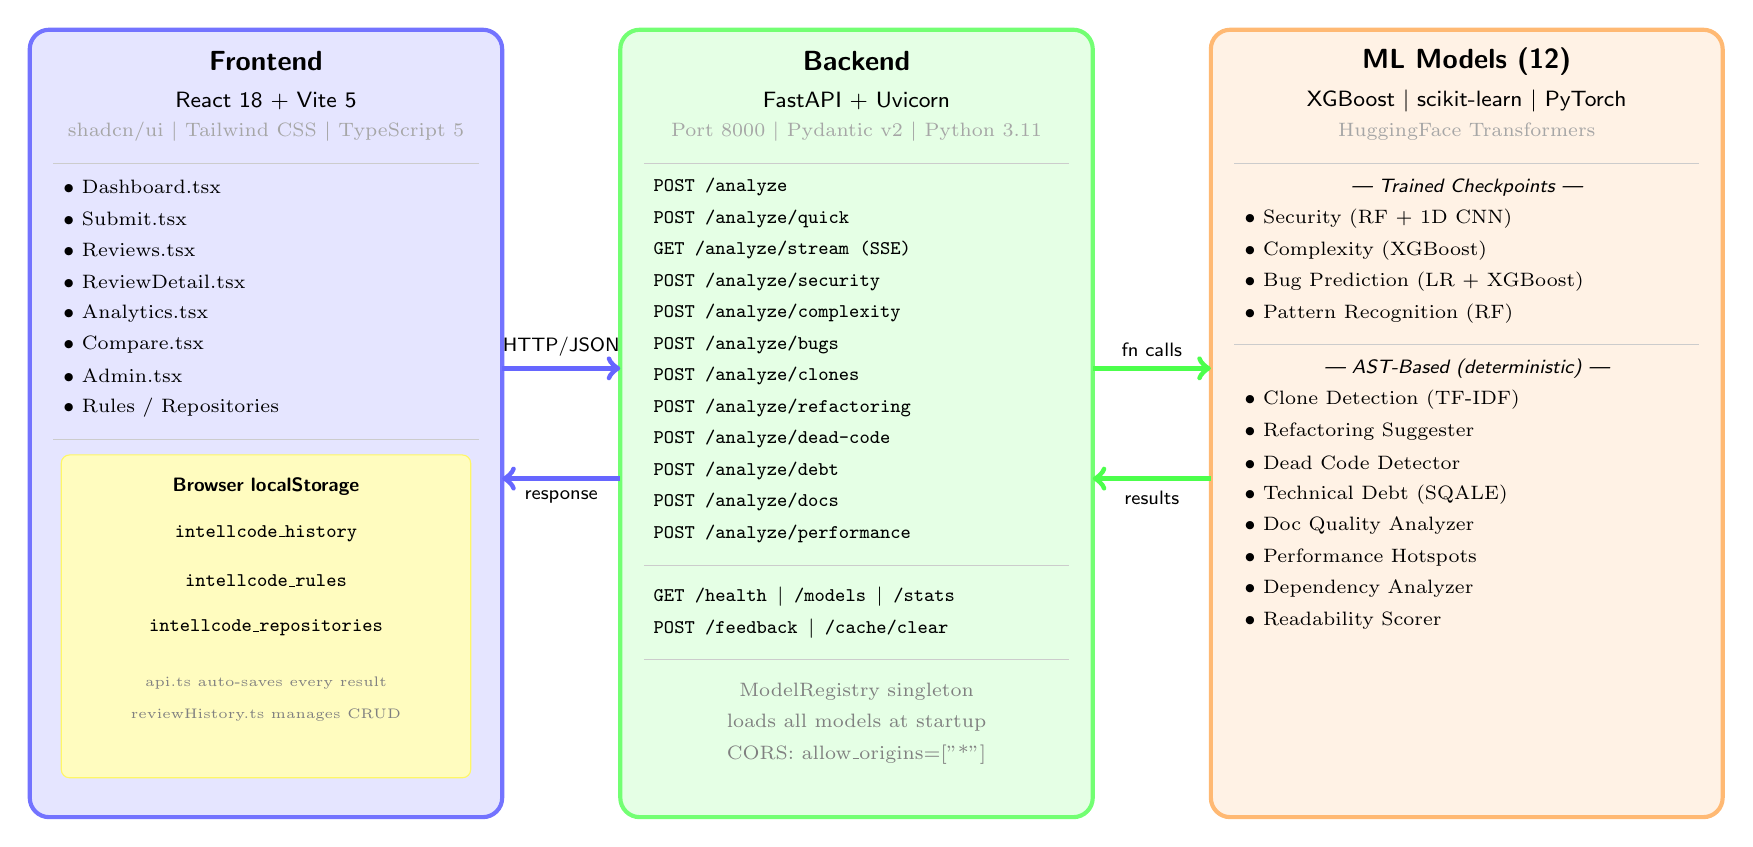
\begin{tikzpicture}[font=\sffamily\footnotesize]

%% ─── Frontend box ───────────────────────────────────────────
\filldraw[fill=blue!10, draw=blue!55, line width=1.5pt, rounded corners=7pt]
  (-3.0,-5.0) rectangle (3.0,5.0);
\node[font=\sffamily\bfseries\normalsize] at (0,4.6) {Frontend};
\node at (0,4.1) {React 18 + Vite 5};
\node[font=\scriptsize, text=gray!70] at (0,3.7) {shadcn/ui \textbar\ Tailwind CSS \textbar\ TypeScript 5};
\draw[gray!40, thin] (-2.7,3.3) -- (2.7,3.3);
\node[font=\scriptsize, anchor=west] at (-2.7, 3.0) {$\bullet$~Dashboard.tsx};
\node[font=\scriptsize, anchor=west] at (-2.7, 2.6) {$\bullet$~Submit.tsx};
\node[font=\scriptsize, anchor=west] at (-2.7, 2.2) {$\bullet$~Reviews.tsx};
\node[font=\scriptsize, anchor=west] at (-2.7, 1.8) {$\bullet$~ReviewDetail.tsx};
\node[font=\scriptsize, anchor=west] at (-2.7, 1.4) {$\bullet$~Analytics.tsx};
\node[font=\scriptsize, anchor=west] at (-2.7, 1.0) {$\bullet$~Compare.tsx};
\node[font=\scriptsize, anchor=west] at (-2.7, 0.6) {$\bullet$~Admin.tsx};
\node[font=\scriptsize, anchor=west] at (-2.7, 0.2) {$\bullet$~Rules / Repositories};
\draw[gray!40, thin] (-2.7,-0.2) -- (2.7,-0.2);
\filldraw[fill=yellow!25, draw=yellow!60, rounded corners=3pt]
  (-2.6,-0.4) rectangle (2.6,-4.5);
\node[font=\sffamily\bfseries\scriptsize] at (0,-0.8) {Browser localStorage};
\node[font=\scriptsize\ttfamily] at (0,-1.4) {intellcode\_history};
\node[font=\scriptsize\ttfamily] at (0,-2.0) {intellcode\_rules};
\node[font=\scriptsize\ttfamily] at (0,-2.6) {intellcode\_repositories};
\node[font=\tiny, text=gray] at (0,-3.3) {api.ts auto-saves every result};
\node[font=\tiny, text=gray] at (0,-3.7) {reviewHistory.ts manages CRUD};

%% ─── Backend box ────────────────────────────────────────────
\filldraw[fill=green!10, draw=green!55, line width=1.5pt, rounded corners=7pt]
  (4.5,-5.0) rectangle (10.5,5.0);
\node[font=\sffamily\bfseries\normalsize] at (7.5,4.6) {Backend};
\node at (7.5,4.1) {FastAPI + Uvicorn};
\node[font=\scriptsize, text=gray!70] at (7.5,3.7) {Port 8000 \textbar\ Pydantic v2 \textbar\ Python 3.11};
\draw[gray!40, thin] (4.8,3.3) -- (10.2,3.3);
\node[font=\ttfamily\scriptsize, anchor=west] at (4.8,3.0) {POST /analyze};
\node[font=\ttfamily\scriptsize, anchor=west] at (4.8,2.6) {POST /analyze/quick};
\node[font=\ttfamily\scriptsize, anchor=west] at (4.8,2.2) {GET  /analyze/stream (SSE)};
\node[font=\ttfamily\scriptsize, anchor=west] at (4.8,1.8) {POST /analyze/security};
\node[font=\ttfamily\scriptsize, anchor=west] at (4.8,1.4) {POST /analyze/complexity};
\node[font=\ttfamily\scriptsize, anchor=west] at (4.8,1.0) {POST /analyze/bugs};
\node[font=\ttfamily\scriptsize, anchor=west] at (4.8,0.6) {POST /analyze/clones};
\node[font=\ttfamily\scriptsize, anchor=west] at (4.8,0.2) {POST /analyze/refactoring};
\node[font=\ttfamily\scriptsize, anchor=west] at (4.8,-0.2) {POST /analyze/dead-code};
\node[font=\ttfamily\scriptsize, anchor=west] at (4.8,-0.6) {POST /analyze/debt};
\node[font=\ttfamily\scriptsize, anchor=west] at (4.8,-1.0) {POST /analyze/docs};
\node[font=\ttfamily\scriptsize, anchor=west] at (4.8,-1.4) {POST /analyze/performance};
\draw[gray!40, thin] (4.8,-1.8) -- (10.2,-1.8);
\node[font=\ttfamily\scriptsize, anchor=west] at (4.8,-2.2) {GET  /health \textbar\ /models \textbar\ /stats};
\node[font=\ttfamily\scriptsize, anchor=west] at (4.8,-2.6) {POST /feedback \textbar\ /cache/clear};
\draw[gray!40, thin] (4.8,-3.0) -- (10.2,-3.0);
\node[font=\scriptsize, text=gray] at (7.5,-3.4) {ModelRegistry singleton};
\node[font=\scriptsize, text=gray] at (7.5,-3.8) {loads all models at startup};
\node[font=\scriptsize, text=gray] at (7.5,-4.2) {CORS: allow\_origins=["*"]};

%% ─── ML Models box ──────────────────────────────────────────
\filldraw[fill=orange!10, draw=orange!55, line width=1.5pt, rounded corners=7pt]
  (12.0,-5.0) rectangle (18.5,5.0);
\node[font=\sffamily\bfseries\normalsize] at (15.25,4.6) {ML Models (12)};
\node at (15.25,4.1) {XGBoost \textbar\ scikit-learn \textbar\ PyTorch};
\node[font=\scriptsize, text=gray!70] at (15.25,3.7) {HuggingFace Transformers};
\draw[gray!40, thin] (12.3,3.3) -- (18.2,3.3);
\node[font=\sffamily\itshape\scriptsize] at (15.25,3.0) {--- Trained Checkpoints ---};
\node[font=\scriptsize, anchor=west] at (12.3,2.6) {$\bullet$~Security (RF + 1D CNN)};
\node[font=\scriptsize, anchor=west] at (12.3,2.2) {$\bullet$~Complexity (XGBoost)};
\node[font=\scriptsize, anchor=west] at (12.3,1.8) {$\bullet$~Bug Prediction (LR + XGBoost)};
\node[font=\scriptsize, anchor=west] at (12.3,1.4) {$\bullet$~Pattern Recognition (RF)};
\draw[gray!40, thin] (12.3,1.0) -- (18.2,1.0);
\node[font=\sffamily\itshape\scriptsize] at (15.25,0.7) {--- AST-Based (deterministic) ---};
\node[font=\scriptsize, anchor=west] at (12.3, 0.3) {$\bullet$~Clone Detection (TF-IDF)};
\node[font=\scriptsize, anchor=west] at (12.3,-0.1) {$\bullet$~Refactoring Suggester};
\node[font=\scriptsize, anchor=west] at (12.3,-0.5) {$\bullet$~Dead Code Detector};
\node[font=\scriptsize, anchor=west] at (12.3,-0.9) {$\bullet$~Technical Debt (SQALE)};
\node[font=\scriptsize, anchor=west] at (12.3,-1.3) {$\bullet$~Doc Quality Analyzer};
\node[font=\scriptsize, anchor=west] at (12.3,-1.7) {$\bullet$~Performance Hotspots};
\node[font=\scriptsize, anchor=west] at (12.3,-2.1) {$\bullet$~Dependency Analyzer};
\node[font=\scriptsize, anchor=west] at (12.3,-2.5) {$\bullet$~Readability Scorer};

%% ─── Arrows ─────────────────────────────────────────────────
\draw[->, line width=2pt, draw=blue!60]
  (3.0, 0.7) -- (4.5, 0.7)
  node[midway, above, font=\scriptsize\sffamily] {HTTP/JSON};
\draw[<-, line width=2pt, draw=blue!60]
  (3.0,-0.7) -- (4.5,-0.7)
  node[midway, below, font=\scriptsize\sffamily] {response};
\draw[->, line width=2pt, draw=green!70]
  (10.5, 0.7) -- (12.0, 0.7)
  node[midway, above, font=\scriptsize\sffamily] {fn calls};
\draw[<-, line width=2pt, draw=green!70]
  (10.5,-0.7) -- (12.0,-0.7)
  node[midway, below, font=\scriptsize\sffamily] {results};

\end{tikzpicture}%
}
\caption{High-level architecture of IntelliCode Review.}
\label{fig:architecture}
\end{figure}

%% ============================================================
\chapter{Software Design and Implementation}
\label{ch:design}
%% ============================================================

\section{Requirements Specification}
\label{sec:requirements}

The functional requirements for IntelliCode Review were derived from the three
research questions and the design goals stated in Chapter~\ref{ch:motivation}. Twelve
primary use cases were identified, which together cover the full range of interactions a
developer would have with the platform (Table~\ref{tab:usecases}).

\begin{table}[H]
\centering
\caption{Use cases for IntelliCode Review}
\label{tab:usecases}
\begin{tabular}{@{}clp{8.5cm}@{}}
\toprule
\textbf{ID} & \textbf{Actor} & \textbf{Description} \\
\midrule
UC01 & Developer & Submit Python, JavaScript, TypeScript, or Java source code and receive a full quality report \\
UC02 & Developer & Inspect the detailed analysis report across all twelve dimensions \\
UC03 & Developer & View a guided fix recommendation for each detected vulnerability \\
UC04 & Developer & Compare two code snippets side by side to evaluate refactoring impact \\
UC05 & Developer & Track quality trends across multiple submissions over time \\
UC06 & Developer & Configure and preview custom quality rules \\
UC07 & Developer & Connect a GitHub repository and initiate a batch scan \\
UC08 & Developer & Export an analysis report as a Markdown document \\
UC09 & Developer & Receive a browser notification when a critical security issue is found \\
UC10 & Developer & Use keyboard shortcuts for common actions without leaving the editor \\
UC11 & Admin & Monitor ML model status, backend statistics, and flush the result cache \\
UC12 & Admin & Collect and review developer feedback submitted on individual analyses \\
\bottomrule
\end{tabular}
\end{table}

Non-functional requirements were formulated alongside the functional requirements.
Full analysis of a 1000-line Python file must complete within two seconds; the fast
endpoint must respond within 500\,ms. The interface must be fully responsive for
desktop resolutions of 1280 pixels and wider. All analysis history, rules, and
repository configurations must persist across browser sessions without a server-side
database. Every finding must be accompanied by a severity classification and a
concrete, human-readable recommendation.

\section{System Architecture}
\label{sec:arch}

IntelliCode Review follows a classical three-tier web architecture with a strict separation
of concerns. The React single-page application running in the browser communicates
with the Python FastAPI backend exclusively over HTTP/JSON; no shared in-memory state
exists between the two tiers. The FastAPI layer in turn invokes a collection of ML model
objects that are loaded once at server startup and held in a singleton
\texttt{ModelRegistry}, ensuring that model load time is not incurred on
every request. This design decouples the analysis logic entirely from HTTP handling,
making individual models testable and replaceable without modifying the API layer.

The frontend, backend, and ML model layer correspond to the three boxes in
Figure~\ref{fig:architecture}. Within the frontend, all persistence is managed via the
browser's \texttt{localStorage} API; a typed TypeScript service layer (\texttt{api.ts},
\texttt{reviewHistory.ts}, \texttt{auth.ts}) abstracts HTTP calls and storage reads so
that page components contain no direct network or storage logic. Within the backend,
an in-memory hash-keyed cache (maximum 200 entries) is consulted before running
models, avoiding redundant computation on repeated identical submissions.

\section{Feature Extraction Layer}
\label{sec:features}

Feature extraction is the shared foundation on which both the ML models and the
deterministic analysers operate. Three modules provide reusable computation that is
invoked once per analysis request and whose results are passed downstream to all
twelve model classes.

\subsection{Multi-Language Adapter}

The \texttt{compute\_metrics\_for\_language()} function dispatches to a language-aware
backend based on the file extension or an explicit language hint. Python submissions
use the \texttt{ast}-based extractor described below. JavaScript, TypeScript, and Java
submissions are parsed with tree-sitter~\cite{tree-sitter} using language-specific
grammars (\texttt{tree-sitter-javascript}, \texttt{tree-sitter-typescript},
\texttt{tree-sitter-java}). For these languages, the adapter computes the same
15-dimensional metric vector (SLOC, comment lines, Halstead approximations, cyclomatic
complexity, cognitive complexity, and line-length statistics) using iterative tree-sitter
AST walks. The resulting \texttt{CodeMetricsResult} object is type-compatible with the
Python path, allowing downstream models to consume it without modification. ML models
that require Python-specific features (bug prediction, pattern recognition) fall back to
rule-based defaults for non-Python code.

\subsection{AST Extractor}

The \texttt{ASTExtractor} class parses Python source code using the standard
\texttt{ast} module and walks the resulting tree in a single pass, collecting function
and class definitions (names, line ranges, parameter counts, decorator lists), import
statements, call sites, string literals, and control-flow construct counts. The nesting
depth of control-flow blocks is tracked as a running maximum during the traversal.
A secondary tokenisation pathway produces integer token-ID sequences of length 512
(padded or truncated), which serve as input to the 1D CNN security component; the
vocabulary used for this mapping is constructed once during training and persisted
alongside the model checkpoints.

\subsection{Code Metrics}

The \texttt{compute\_all\_metrics()} function computes a 17-dimensional feature vector
that is shared across the complexity, security, and bug prediction models. The most
theoretically grounded metrics in this vector are cyclomatic complexity and the
Maintainability Index:

\begin{align}
  V(G) &= E - N + 2P \quad \text{(cyclomatic complexity)} \label{eq:cc}\\
  MI &= 171 - 5.2 \ln(HV) - 0.23 V(G) - 16.2 \ln(SLOC) \label{eq:mi}
\end{align}

where $HV$ is Halstead volume, $V(G)$ is cyclomatic complexity, and $SLOC$ is source
lines of code. The Maintainability Index (\ref{eq:mi}) is scaled to [0, 100] and
serves as the target variable for the XGBoost complexity model.

Cognitive complexity is computed by incrementing a counter for each control flow
branching point, with additional penalty increments for each level of nesting:

\begin{equation}
  CC = \sum_{i} (1 + \text{nesting\_depth}(i)) \label{eq:cogcomplexity}
\end{equation}

\subsection{Security Pattern Scanner}

The \texttt{scan\_security\_patterns()} function implements a regular-expression-based
vulnerability scanner covering eight vulnerability categories (Table~\ref{tab:vulntypes}).
Each category has associated CWE identifiers and severity classifications (critical, high,
medium, low). The scanner runs on every analysis request and its findings serve both as
direct output and as features for the ML ensemble.

\begin{table}[H]
\centering
\caption{Security vulnerability categories detected by IntelliCode Review}
\label{tab:vulntypes}
\begin{tabular}{@{}lll@{}}
\toprule
\textbf{Category} & \textbf{CWE} & \textbf{Severity} \\
\midrule
SQL Injection           & CWE-89  & Critical \\
Command Injection       & CWE-78  & Critical \\
Hardcoded Secret        & CWE-798 & Critical \\
Insecure Deserialization & CWE-502 & Critical \\
Path Traversal          & CWE-22  & High \\
Weak Cryptography       & CWE-327 & High \\
Code Injection (eval)   & CWE-94  & High \\
XML External Entity     & CWE-611 & Medium \\
\bottomrule
\end{tabular}
\end{table}

\section{Machine Learning Models}
\label{sec:models}

\subsection{Security Vulnerability Detection: RF + 1D CNN Ensemble}
\label{ssec:security}

The security detection model (\texttt{security\_detection.py}) uses an ensemble of two
complementary classifiers. The feature vector for the Random Forest has 25 dimensions:
the 17 code metrics from \texttt{code\_metrics.py} plus 8 security-specific counters
(dangerous import count, dangerous call count, long string count, scanner findings at
each severity level, try block count, string literal count, call site count).

The 1D CNN operates on a padded/truncated sequence of 512 integer token IDs. Its
architecture is:

\begin{equation}
  \text{TextCNN}: \text{Embed}_{10000 \to 128} \to
  \underbrace{\text{Conv1d}_{k \in \{3,5,7\}} \to \text{ReLU} \to \text{MaxPool}}_{\times 3}
  \to \text{Concat} \to \text{Dropout}_{0.5} \to \text{Linear}_{768 \to 2}
\end{equation}

The ensemble combines both components:
\begin{equation}
  p_{\text{vuln}} = \frac{w_{RF} \cdot p_{RF} + w_{CNN} \cdot p_{CNN}}{w_{RF} + w_{CNN}},
  \quad w_{RF} = 0.55,\; w_{CNN} = 0.45
\end{equation}

The Random Forest uses 200 trees with Platt scaling for probability calibration
(\texttt{CalibratedClassifierCV}, \texttt{cv=5}, \texttt{method='sigmoid'}).

\subsection{Complexity Prediction: XGBoost}
\label{ssec:complexity}

The complexity model (\texttt{complexity\_prediction.py}) is an XGBoost regressor
predicting a maintainability score in $[0, 100]$ from the 17-dimensional feature vector.
The score is capped to $[0, 100]$ and mapped to letter grades:

\begin{table}[H]
\centering
\caption{Complexity grade thresholds}
\label{tab:grades}
\begin{tabular}{@{}ll@{}}
\toprule
\textbf{Score Range} & \textbf{Grade} \\
\midrule
$\geq 80$ & A (Excellent) \\
$\geq 65$ & B (Good) \\
$\geq 50$ & C (Fair) \\
$\geq 35$ & D (Poor) \\
$< 35$ & F (Critical) \\
\bottomrule
\end{tabular}
\end{table}

Beyond the scalar score, the model identifies specific problem functions: functions
with cyclomatic complexity $> 10$, body length $> 50$ lines, or parameter count $> 5$
are flagged with specific recommendations (``Reduce complexity'', ``Extract sub-functions'',
``Reduce parameters'').

\subsection{Bug Prediction: Logistic Regression + XGBoost Ensemble}
\label{ssec:bugs}

The bug predictor (\texttt{bug\_predictor.py}) combines static code features with optional
git metadata. The static feature vector is the same 17-dimensional code metrics vector.
Git metadata (when provided) adds 5 features: code churn, author count, file age in days,
past bug count, and commit frequency.

The Logistic Regression component uses the full 22-dimensional combined vector. The XGBoost
component is a gradient-boosted classifier trained with early stopping (best iteration at
epoch 97, preventing overfitting beyond that point). The ensemble averages LR and XGBoost
probabilities:

\begin{equation}
  p_{\text{bug}} = \frac{p_{LR} + p_{XGB}}{2}
\end{equation}

Training was performed on 8668 real OSS commit records labelled via keyword-based SZZ
heuristics (commit messages containing ``fix'' or ``bug''), with \texttt{is\_fix} excluded
from features to prevent circular labels. Held-out AUC scores: LR = 0.682 (multi-seed
$0.676 \pm 0.038$), XGB = 0.934 (circular on keyword labels). Cross-project LOPO AUC
$= 0.567 \pm 0.028$; 5-fold walk-forward temporal CV AUC $= 0.544 \pm 0.105$.
A heuristic fallback is used when checkpoints are unavailable, based on thresholds applied
directly to cyclomatic complexity and Halstead bugs metrics.

Risk levels are classified as:
\begin{itemize}
  \item \textbf{Critical}: $p > 0.75$
  \item \textbf{High}: $0.50 < p \leq 0.75$
  \item \textbf{Medium}: $0.25 < p \leq 0.50$
  \item \textbf{Low}: $p \leq 0.25$
\end{itemize}

\subsection{Pattern Recognition: Calibrated Random Forest}
\label{ssec:pattern}

The pattern recognition model (\texttt{pattern\_recognition.py}) is a Random Forest
classifier with 300 trees trained on a \textbf{12-dimensional debiased AST feature
vector}. The four output classes are: \texttt{clean}, \texttt{code\_smell},
\texttt{anti\_pattern}, and \texttt{style\_violation}. Probability calibration is applied
via Platt scaling (\texttt{CalibratedClassifierCV}, \texttt{method='sigmoid'},
\texttt{cv=5}), which improves the reliability of per-class confidence scores reported to
the frontend.

A label leakage analysis (Section~\ref{ssec:pattern-leakage}) identified that the
original 26-feature set included CC, SLOC, Halstead volume, and related metrics that are
also used as inputs to the label assignment rules, creating circular self-supervision.
The 14 leaky features were removed, leaving 12 structural AST features (function counts,
class/block counts, nesting depth, parameter statistics) that are genuinely independent of
the labeling thresholds. The model was trained on 1153 real OSS code samples.
Evaluation on the held-out test split yields:
\textbf{accuracy = 66.5\%}, \textbf{AUC = 0.846}, and cross-validated F1 = 0.657.
The leaky 26-feature model achieved 80.3\% accuracy and 0.969 AUC---a confirmed
$+0.082$ F1 inflation (Wilcoxon $p=0.031$, significant at $\alpha=0.05$).
The debiased checkpoint (\texttt{checkpoints/pattern/rf\_model.pkl}) loads
in under 100\,ms at startup.

\subsection{Code Clone Detection: TF-IDF Cosine Similarity}
\label{ssec:clones}

The clone detector (\texttt{code\_clone\_detection.py}) extracts function bodies from the
submitted code, normalizes them (stripping comments, whitespace, and optionally renaming
identifiers for Type-2 detection), and computes pairwise TF-IDF cosine similarity.
Function pairs with similarity above $0.85$ (Type-1), $0.70$ (Type-2), or $0.55$ (Type-3)
thresholds are reported as clones. The result includes clone pairs, their type
classification, and similarity scores.

\subsection{Refactoring Suggester: AST Rule Engine}
\label{ssec:refactoring}

The refactoring suggester applies a set of threshold-based AST rules derived from
established refactoring catalogues~\cite{fowler1999}. Functions exceeding 40 lines
are flagged for method extraction; nesting depth greater than three levels triggers
a reduce-nesting suggestion; boolean expressions with more than four operators are
candidates for simplification. Three further rules target identifier clarity (overly
abbreviated names), type annotation coverage (unannotated public APIs), and
parameter count (more than five arguments). Each suggestion carries an estimated
remediation effort in minutes and a priority score used to rank the output list.

\subsection{Dead Code Detector: AST Definition/Usage Graph}
\label{ssec:deadcode}

The dead code detector (\texttt{dead\_code\_detector.py}) builds definition and usage
sets by walking the AST. It identifies: (1) imported names that are never referenced,
(2) defined functions or classes that are never called or instantiated, (3) code after
\texttt{return} or \texttt{raise} statements (unreachable code), (4) empty \texttt{except}
blocks that swallow exceptions silently, and (5) variables assigned but never read.
Each finding includes line number, symbol name, and dead code category.

\subsection{Technical Debt Estimator: SQALE-Inspired Aggregator}
\label{ssec:debt}

The technical debt estimator (\texttt{technical\_debt.py}) aggregates findings from all
other models into a debt report following the SQALE methodology~\cite{letouzey2012}.
Debt is estimated in minutes of remediation effort per finding (Table~\ref{tab:debtrates})
and summed into category totals. The overall debt rating (A--E) is determined by the
ratio of total debt to estimated development time.

\begin{table}[H]
\centering
\caption{Technical debt remediation rates used by the estimator}
\label{tab:debtrates}
\begin{tabular}{@{}lrr@{}}
\toprule
\textbf{Category} & \textbf{Minutes/Finding} & \textbf{Max Minutes} \\
\midrule
Critical security finding & 120 & --- \\
High security finding     &  60 & --- \\
Complexity (score $< 60$) &  30 & --- \\
Bug risk (High/Critical)  &  45 & --- \\
Code clone                &  20 & 240 \\
Dead code finding         &  10 & 120 \\
Refactoring suggestion    &  15 & 180 \\
\bottomrule
\end{tabular}
\end{table}

\subsection{Documentation Quality Analyzer}
\label{ssec:docs}

The documentation analyzer (\texttt{doc\_quality\_analyzer.py}) walks the AST collecting
all function and class definitions and examining their docstrings. It computes:
(1) docstring coverage (fraction of public functions/classes with docstrings),
(2) docstring completeness (presence of parameter, return, and raises sections),
(3) docstring length adequacy (minimum one sentence), and (4) overall quality grade (A--F).
Functions and classes lacking docstrings or having inadequate ones are reported individually.

\subsection{Performance Hotspot Predictor}
\label{ssec:performance}

The performance analyser detects AST patterns that correspond to well-known Python
performance anti-patterns: nested loops (O($n^2$) complexity risk), string
concatenation inside loops (quadratic memory allocation from repeated object
creation), I/O calls inside loops, mutable default arguments (shared state across
invocations), list comprehensions where generator expressions would suffice, and
global variable access in hot paths. Because these patterns are detectable
syntactically without execution, false negative rates are low, though interprocedural
patterns (e.g., a loop in one function calling an I/O-heavy function in another)
remain outside the scope of single-file static analysis.

\subsection{Dependency and Coupling Analyzer}
\label{ssec:dependency}

The dependency analyser constructs a module-level import graph from the AST and
derives three coupling indicators. Fan-out counts the number of distinct imported
modules, providing a rough measure of efferent coupling. Instability is computed as
$I = C_e / (C_e + C_a)$, where $C_e$ is efferent coupling and $C_a$ is afferent
coupling approximated from repeated imports of the same module across the code
under analysis. Wildcard imports (\texttt{from~module~import~*}) are flagged
separately because they pollute the local namespace in a way that makes dead-code
analysis unreliable and is classified as CWE-1104 (use of unmaintained third-party
components). These three indicators are combined into a composite coupling score
(0--100, higher is worse) that surfaces in the dependency tab of the review detail
page.

\subsection{Code Readability Scorer}
\label{ssec:readability}

The readability scorer is inspired by the Buse and Weimer~\cite{buse2010} feature
set but extends it to four distinct sub-dimensions, each contributing up to 25 points
to an overall score of 100. Naming quality rewards adequate identifier length and
consistent \texttt{snake\_case} convention while penalising single-character names
beyond conventional loop counters. Comment quality measures comment density,
the ratio of inline to block comments, and the presence of section-level headers.
Structural quality evaluates function length distribution, control-flow nesting depth,
and blank-line separation. Finally, cognitive load penalises deeply nested boolean
expressions, magic number literals, and excessively long lines. The four sub-scores
are summed and mapped to an A--F grade using the same thresholds as the complexity
model, enabling a consistent grading language across all scoring dimensions.

\section{Training Pipeline}
\label{sec:training}

\subsection{Real Dataset Construction}

IntelliCode Review's training data is sourced from real open-source Python projects rather
than synthetic generation. The \texttt{fetch\_real\_datasets.py} script collects samples
from the following sources:

\begin{itemize}
  \item \textbf{Complexity dataset (3000 samples)}: Python functions extracted from the
    Django, Flask, and requests repositories. Maintainability scores are computed
    analytically from the AST using \texttt{code\_metrics.py}, yielding ground-truth
    regression targets that reflect real code structure distributions.
  \item \textbf{Security dataset (3000 samples)}: Balanced mix of (a) clean functions
    from the same OSS repos and (b) vulnerable samples from CVE-annotated commits and
    Bandit-labelled examples. Label: binary (0 = clean, 1 = vulnerable).
  \item \textbf{Bug dataset (3000 samples)}: Functions from Django and pip, labelled via
    SZZ-style heuristics (commits containing ``fix'', ``bug'', or ``error'' keywords in the
    message). Label: binary (0 = low risk, 1 = high risk).
  \item \textbf{Pattern dataset (1825 samples)}: Code blocks labelled with one of four
    categories (clean, god\_class, long\_method, feature\_envy) using structural
    heuristics: classes with $> 10$ methods are labelled \texttt{god\_class}; functions
    with $> 40$ lines are labelled \texttt{long\_method}; functions with high fan-out
    coupling are labelled \texttt{feature\_envy}.
\end{itemize}

\subsection{Model Training}

The master training script \texttt{train\_all.py} orchestrates five training steps:

\begin{enumerate}
  \item \textbf{Data collection}: calls \texttt{fetch\_real\_datasets.py} to download
    and label JSONL files in \texttt{backend/data/}.
  \item \textbf{Complexity training} (\texttt{train\_complexity.py}): fits an XGBoost
    regressor on the complexity dataset with 80/20 train/test split. The prediction
    target is cognitive complexity (not Maintainability Index, which would cause target
    leakage as it is a closed-form function of features already in the input vector).
    Post-audit result: $R^2 = 0.712$, RMSE = 49.5, Spearman $\rho = 0.865$.
  \item \textbf{Security training} (\texttt{train\_security.py}): trains the Random Forest
    (200 trees, Platt calibration) on the security dataset. Multi-seed evaluation
    (5 seeds) yields AUC $= 0.834 \pm 0.036$, AP $= 0.680 \pm 0.057$.
    Cross-project LOPO AUC $= 0.494 \pm 0.189$ confirms near-chance generalisation.
  \item \textbf{Bug training} (\texttt{train\_bugs.py}): trains the XGBoost bug predictor
    on the bug dataset. Multi-seed evaluation (5 seeds) yields AUC $= 0.676 \pm 0.038$.
    5-fold walk-forward temporal cross-validation yields mean AUC $= 0.544 \pm 0.105$
    versus random-split AUC $= 0.676$ ($\Delta\text{AUC} = -0.132$), confirming
    temporal data leakage. The per-fold variance ($\pm0.105$) is itself informative:
    it shows the model's performance depends strongly on which time period is used
    as the test window, which a single 70/30 cut obscures.
  \item \textbf{Pattern training} (\texttt{train\_pattern.py}): trains the calibrated
    Random Forest (300 trees, Platt scaling, \texttt{cv=5}) on the 1153-sample pattern
    dataset using 12 debiased structural AST features. Cross-validation uses
    \texttt{n\_jobs=1} on Windows to avoid shared-memory serialisation errors.
    Debiased result: accuracy = 66.5\%, AUC = 0.846, CV F1 = $0.657 \pm 0.016$.
    The prior 26-feature model (accuracy = 80.3\%, AUC = 0.969) is deprecated due
    to confirmed label leakage ($+0.082$ F1 inflation, Wilcoxon $p=0.031$).
\end{enumerate}

Checkpoints are saved in \texttt{backend/checkpoints/} as pickle files (\texttt{.pkl}
for scikit-learn and XGBoost models) and PyTorch state dicts (\texttt{.pt} files for the
1D CNN). Each model directory also stores a \texttt{metrics.json} file recording final
evaluation metrics and (for security) the optimal classification threshold.

\section{Backend API}
\label{sec:api}

The FastAPI application (\texttt{main.py}) defines the model registry as a singleton
class (\texttt{ModelRegistry}) that is populated during the application startup lifespan:

\begin{lstlisting}[caption={FastAPI lifespan: loading ML models at startup},
                   label={lst:lifespan}, style=pythonstyle]
@asynccontextmanager
async def lifespan(app: FastAPI):
    """Load models on startup."""
    print("Loading ML models...")
    try:
        registry.security = EnsembleSecurityModel(
            checkpoint_dir="checkpoints/security")
        print("  [OK] Security detection model")
    except Exception as e:
        registry.load_errors["security"] = str(e)
    # ... (other models loaded similarly)
    registry.clone_detector = CodeCloneDetector()
    registry.refactoring_suggester = RefactoringSuggester()
    # ... (all lightweight models always load)
    yield
    print("Shutting down.")
\end{lstlisting}

The combined analysis endpoint (\texttt{POST /analyze}) accepts a JSON payload with fields
\texttt{code}, \texttt{filename}, \texttt{language}, and optional \texttt{git\_metadata},
and returns a \texttt{FullAnalysisResponse} JSON object containing results from all twelve
models plus an \texttt{overall\_score} (0--100) and a \texttt{status} field (``clean'',
``action\_required'', or ``critical''). Results are cached in a hash-keyed in-memory
dictionary (maximum 200 entries) to avoid re-running expensive models on repeated
identical submissions.

Three additional analysis endpoints extend the core capability:

\begin{itemize}
  \item \texttt{POST /analyze/quick} — runs only security pattern scanning, complexity
    metrics, and readability scoring, returning a lightweight result in under 500\,ms.
    This endpoint is suitable for IDE integrations or CI pre-commit hooks where full
    analysis latency is prohibitive.
  \item \texttt{GET /analyze/stream} — a Server-Sent Events (SSE) endpoint that streams
    partial analysis results as each model completes. The frontend \texttt{EventSource}
    connection receives named events (\texttt{security}, \texttt{complexity}, \texttt{bugs},
    etc.) and updates the UI progressively, providing live feedback during long analyses.
\end{itemize}

Three utility endpoints support operations and monitoring:

\begin{itemize}
  \item \texttt{GET /stats} — returns aggregate statistics computed from the in-memory
    cache: total analyses served, average quality score, total security findings, and
    number of ready models. Used by the Admin page dashboard cards.
  \item \texttt{POST /feedback} — accepts structured developer feedback
    (\texttt{result\_id}, \texttt{rating} 1--5, optional \texttt{comment}), stored in
    a server-side list for future model improvement analysis.
  \item \texttt{POST /cache/clear} — flushes the analysis result cache, accessible from
    the Admin page.
\end{itemize}

\ac{CORS} is configured to allow all origins (\texttt{allow\_origins=["*"]}), which is
appropriate for a local prototype but should be restricted to the frontend origin in
production.

\section{Frontend Implementation}
\label{sec:frontend}

The frontend is a React~18 single-page application built with Vite and TypeScript,
using React Router~v6 for client-side routing. Eleven pages are accessible from a
persistent sidebar: Dashboard, Submit, Reviews, Review Detail, Compare, Analytics,
Models, Rules, Repositories, Admin, and Settings. A \texttt{ProtectedRoute} component
redirects unauthenticated users to the Login page, and a live API status indicator
polls \texttt{GET /health} every 15 seconds. Analysis history is persisted entirely in
\texttt{localStorage} via \texttt{reviewHistory.ts}, keyed on \texttt{intellcode\_history},
so results survive browser sessions without a server-side database.

The Review Detail page organises results into fourteen tabs (see
Table~\ref{tab:tabs}). Two design choices are architecturally significant. First,
the \texttt{/analyze/stream} SSE endpoint populates the Security tab within the first
200\,ms while remaining models continue asynchronously, reducing perceived latency on
long files. Second, the Fix Guide tab (Tab~14) provides ready-to-paste corrected code
for the five most common vulnerability types, eliminating the context-switch to an
external search. Full per-page component documentation is in
Appendix~\ref{app:frontend}.

\begin{table}[H]
\centering
\caption{Review Detail page tabs}
\label{tab:tabs}
\begin{tabular}{@{}lll@{}}
\toprule
\textbf{\#} & \textbf{Tab} & \textbf{Content} \\
\midrule
1  & Overview       & Score gauge, status, summary metrics \\
2  & Security       & Findings by severity, CWE, line, snippet \\
3  & Complexity     & Score gauge, grade, metric breakdown, flagged functions \\
4  & Bug Risk       & Probability gauge, risk level, contributing factors \\
5  & Pattern        & 4-class RF output with confidence bars \\
6  & Clones         & Detected clone pairs, type, similarity score \\
7  & Refactoring    & Prioritised suggestions with effort estimates \\
8  & Dead Code      & Unused imports, unreachable blocks, empty excepts \\
9  & Tech Debt      & Total debt hours, SQALE rating A--E, per-category \\
10 & Docs           & Coverage \%, grade, undocumented functions \\
11 & Performance    & Anti-patterns with severity and recommended fix \\
12 & Dependencies   & Fan-out, instability, wildcard import warnings \\
13 & Readability    & Score, grade, four sub-dimension scores \\
14 & Fix Guide      & Before/after code blocks with copy buttons for common \\
   &                & vulnerability types (SQL injection, command injection, \\
   &                & hardcoded secrets, XSS, path traversal) \\
\bottomrule
\end{tabular}
\end{table}

\section{Implementation Challenges}
\label{sec:challenges}

Several non-trivial challenges arose during development that merit discussion, as they
reflect design decisions with broader applicability to similar ML-backed web applications.

\subsection{Pydantic v2 Compatibility and Model Output Access}

The backend was originally prototyped against Pydantic v1 idioms, where model output
objects were accessed as dictionaries (\texttt{model.get("field")}). When dependencies
were pinned to Pydantic v2, this pattern silently returned \texttt{None} for every field
because Pydantic v2 output objects are not dicts. The failure manifested only at
runtime during the \texttt{/analyze} endpoint, not at model load time, making it
difficult to isolate. The fix required systematically replacing every dictionary-style
field access with attribute access (\texttt{model.field}) across all model output
handlers in \texttt{main.py}. This experience reinforced the importance of typed
response schemas validated at endpoint boundaries rather than relying on duck typing.

\subsection{Cross-Validation Parallelism on Windows}

scikit-learn's \texttt{cross\_val\_score} defaults to \texttt{n\_jobs=-1}, which
spawns one worker per CPU core using Python's \texttt{multiprocessing} module. On
Windows, the lack of \texttt{fork()} semantics means each worker is spawned via
\texttt{spawn}, requiring every object passed to the worker to be picklable. The
calibrated Random Forest model used for pattern recognition contains closures and
lambda functions that are not safely picklable under this scheme, resulting in silent
out-of-memory crashes on the training machine. The resolution was to set
\texttt{n\_jobs=1} for all cross-validation calls, accepting single-threaded training
in exchange for correctness. This constraint is documented in the training scripts
and represents a known Windows-specific limitation.

\subsection{Streaming Architecture and Browser Compatibility}

Implementing real-time streaming via the \texttt{/analyze/stream} endpoint required
a careful choice of server push technology. WebSockets would have required a
stateful session, complicating the stateless FastAPI architecture. Long-polling was
ruled out due to unnecessary request overhead. Server-Sent Events (SSE) emerged as
the most appropriate mechanism: they operate over standard HTTP/1.1, are natively
supported by the browser \texttt{EventSource} API, and require no additional
WebSocket library on either end. One challenge was that FastAPI's default
\texttt{JSONResponse} is not compatible with streaming; the endpoint was instead
implemented using \texttt{StreamingResponse} with \texttt{text/event-stream} MIME
type and a generator function that yields partial results as each model completes.
The frontend \texttt{EventSource} connection listens for named events and merges
partial results into the accumulating analysis state using React's reducer pattern.

\subsection{Result Cache Invalidation and Memory Bounds}

The in-memory hash-keyed analysis cache posed a memory management challenge: without
bounds, a long-running server instance would accumulate cached results indefinitely.
An LRU-style size limit of 200 entries was chosen as a practical bound, but Python's
built-in \texttt{dict} does not enforce LRU semantics. The cache was implemented
using \texttt{collections.OrderedDict} with manual eviction of the oldest entry when
the limit is reached. The \texttt{POST /cache/clear} endpoint was added to allow
administrators to flush the cache when stale results are suspected, surfaced as a
button on the Admin page.

%% ============================================================
\chapter{Prototype Demonstration}
\label{ch:demo}
%% ============================================================

\section{Interface Overview}
\label{sec:ui-overview}

The IntelliCode Review interface is organised around a persistent sidebar navigation
linking to eleven pages. The landing page presents the platform's value proposition
through a hero section, a feature grid for the twelve analysis dimensions, and an
interactive embedded demo that allows visitors to run a canned analysis before signing
in. Once authenticated, users are directed to the Dashboard, which surfaces a quality
trend sparkline, summary statistics, and a file quality leaderboard.

The Submit page is the primary entry point for analysis. A developer pastes source
code into the editor, optionally enters a filename and language hint, and submits.
The interface was designed to minimise friction: the \textit{Ctrl+Enter} keyboard
shortcut triggers submission from the editor without requiring a mouse click, and a
copy button in the editor chrome allows the current buffer to be transferred to an
external tool in a single action. The backend status indicator embedded in the
navigation bar informs the user at a glance whether the analysis engine is reachable,
preventing confusion when the backend is not running.

\section{Interface Walkthrough}
\label{sec:interface-walkthrough}

\subsection{Dashboard and Analysis History}

After logging in, a developer is presented with the Dashboard. If analyses have been
previously submitted, the dashboard immediately surfaces an area chart of quality scores
over time so that overall trends are visible without navigating to the Analytics page.
When at least two distinct files have been analysed, the leaderboard section renders
two ranked panels: the five highest-scoring files (``Top Quality Files'') and the five
lowest-scoring files (``Needs Attention''). This design was motivated by the observation
that developers working on multiple modules often want to prioritise review effort on
the weakest file rather than the most recently modified one.

\subsection{Code Submission and Streaming}

Figure~\ref{fig:submit} illustrates the Submit page. The developer pastes Python code
into the editor, optionally supplies a filename and language, and submits. A
\texttt{Ctrl+Enter} keyboard shortcut allows submission without releasing the keyboard.
During analysis, the interface optionally streams partial results via the SSE endpoint
(\texttt{/analyze/stream}), displaying each model's findings as it completes rather than
waiting for the full response. This streaming approach was found to substantially reduce
the perceived latency for long files, as the security tab populates within the first
200\,ms while the remaining models continue running.

\begin{figure}[H]
\centering
\resizebox{0.95\linewidth}{!}{%
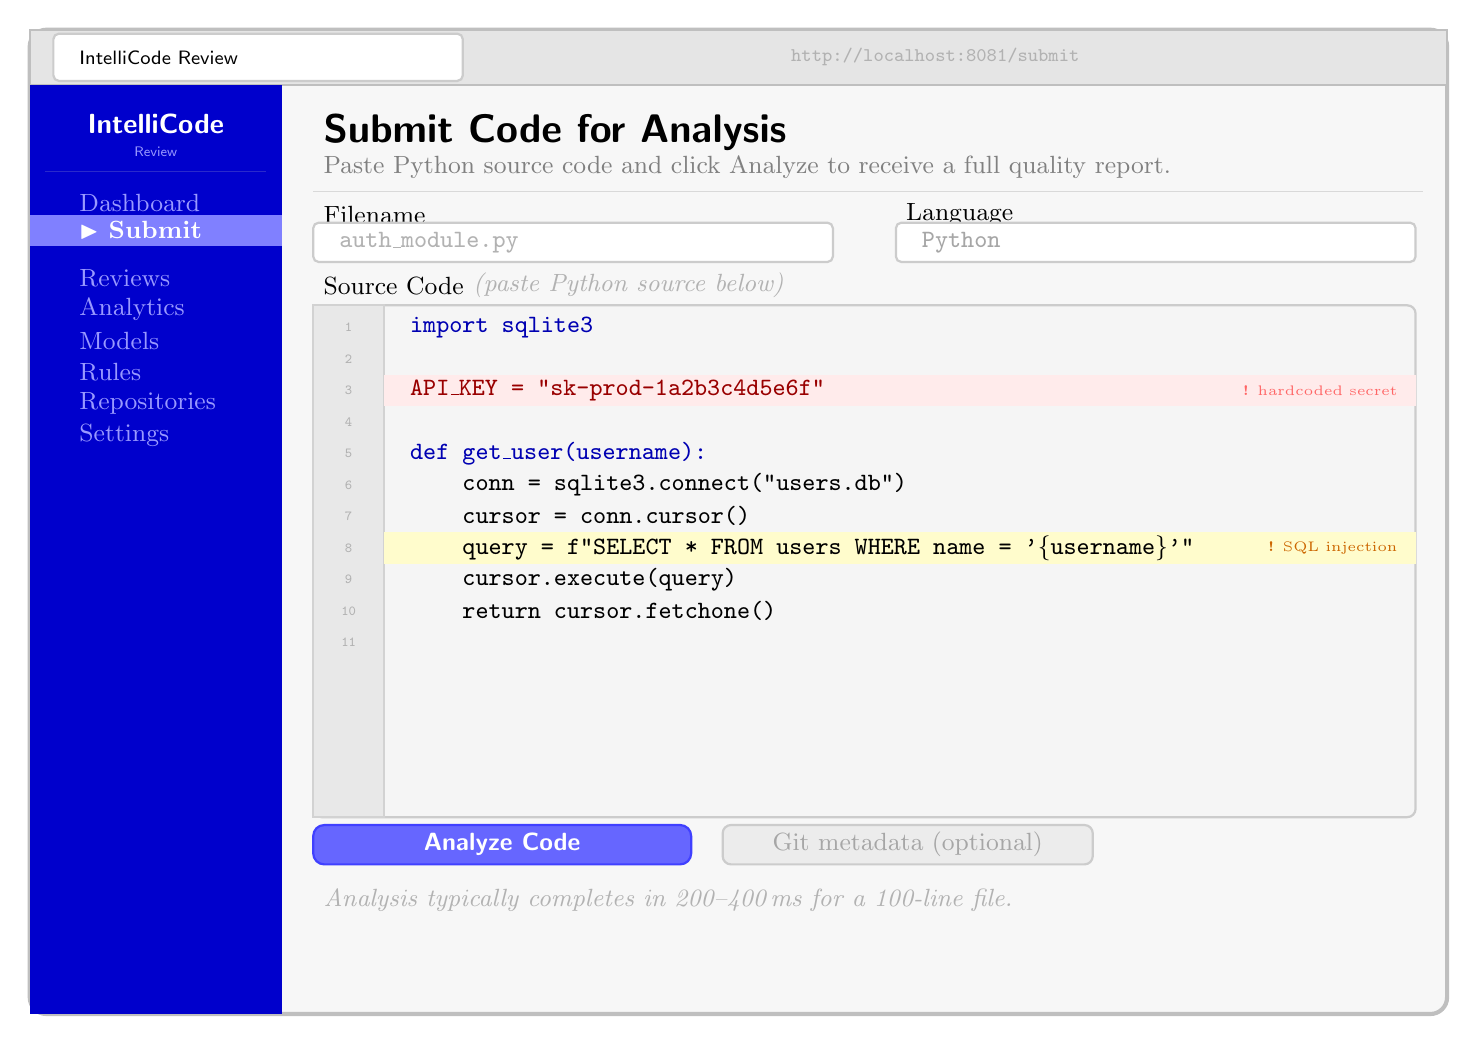
\begin{tikzpicture}[font=\sffamily\normalsize, thick]

%% ─── Window frame ───────────────────────────────────────────
\filldraw[fill=gray!6, draw=gray!50, line width=1.5pt, rounded corners=6pt]
  (0,0) rectangle (18,12.5);

%% ─── Browser tab bar ────────────────────────────────────────
\filldraw[fill=gray!20, draw=gray!50, line width=0.8pt]
  (0,11.8) rectangle (18,12.5);
\draw[fill=white, draw=gray!40, rounded corners=2pt]
  (0.3,11.85) rectangle (5.5,12.45);
\node[font=\sffamily\scriptsize, anchor=west] at (0.5,12.15) {IntelliCode Review};
\node[font=\ttfamily\scriptsize, text=gray!60] at (11.5,12.15)
  {http://localhost:8081/submit};

%% ─── Left sidebar ───────────────────────────────────────────
\filldraw[fill=blue!80!black, draw=none]
  (0,0) rectangle (3.2,11.8);
%% Brand
\node[font=\sffamily\bfseries\normalsize, text=white] at (1.6,11.3) {IntelliCode};
\node[font=\sffamily\tiny, text=blue!40] at (1.6,10.95) {Review};
\draw[white!20!blue!80!black, thin] (0.2,10.7) -- (3.0,10.7);
%% Nav items (inactive)
\node[font=\small, text=blue!40, anchor=west] at (0.5,10.3) {Dashboard};
%% Active item highlight
\filldraw[fill=blue!50, draw=none] (0,9.75) rectangle (3.2,10.15);
\node[font=\small\bfseries, text=white, anchor=west] at (0.5,9.95)
  {$\blacktriangleright$\ Submit};
\node[font=\small, text=blue!40, anchor=west] at (0.5,9.35) {Reviews};
\node[font=\small, text=blue!40, anchor=west] at (0.5,8.95) {Analytics};
\node[font=\small, text=blue!40, anchor=west] at (0.5,8.55) {Models};
\node[font=\small, text=blue!40, anchor=west] at (0.5,8.15) {Rules};
\node[font=\small, text=blue!40, anchor=west] at (0.5,7.75) {Repositories};
\node[font=\small, text=blue!40, anchor=west] at (0.5,7.35) {Settings};

%% ─── Main content ───────────────────────────────────────────
%% Page title
\node[font=\sffamily\bfseries\Large, anchor=west] at (3.6,11.2)
  {Submit Code for Analysis};
\node[font=\small, text=gray, anchor=west] at (3.6,10.75)
  {Paste Python source code and click Analyze to receive a full quality report.};
\draw[gray!30, thin] (3.6,10.45) -- (17.7,10.45);

%% Row 1: Filename + Language fields
\node[font=\small, anchor=west] at (3.6,10.15) {Filename};
\filldraw[fill=white, draw=gray!40, rounded corners=2pt]
  (3.6,9.55) rectangle (10.2,10.05);
\node[font=\small\ttfamily, text=gray!60, anchor=west] at (3.8,9.79)
  {auth\_module.py};
\node[font=\small, anchor=west] at (11.0,10.15) {Language};
\filldraw[fill=white, draw=gray!40, rounded corners=2pt]
  (11.0,9.55) rectangle (17.6,10.05);
\node[font=\small\ttfamily, text=gray!70, anchor=west] at (11.2,9.79)
  {Python};

%% Source code label
\node[font=\small, anchor=west] at (3.6,9.25)
  {Source Code};
\node[font=\small, text=gray!60, anchor=west] at (5.5,9.25)
  {\textit{(paste Python source below)}};

%% Code editor area
\filldraw[fill=gray!8, draw=gray!40, rounded corners=3pt]
  (3.6,2.5) rectangle (17.6,9.0);

%% Editor gutter (line numbers)
\filldraw[fill=gray!18, draw=gray!35]
  (3.6,2.5) rectangle (4.5,9.0);
\node[font=\tiny\ttfamily, text=gray!60] at (4.05,8.72) {1};
\node[font=\tiny\ttfamily, text=gray!60] at (4.05,8.32) {2};
\node[font=\tiny\ttfamily, text=gray!60] at (4.05,7.92) {3};
\node[font=\tiny\ttfamily, text=gray!60] at (4.05,7.52) {4};
\node[font=\tiny\ttfamily, text=gray!60] at (4.05,7.12) {5};
\node[font=\tiny\ttfamily, text=gray!60] at (4.05,6.72) {6};
\node[font=\tiny\ttfamily, text=gray!60] at (4.05,6.32) {7};
\node[font=\tiny\ttfamily, text=gray!60] at (4.05,5.92) {8};
\node[font=\tiny\ttfamily, text=gray!60] at (4.05,5.52) {9};
\node[font=\tiny\ttfamily, text=gray!60] at (4.05,5.12) {10};
\node[font=\tiny\ttfamily, text=gray!60] at (4.05,4.72) {11};

%% Code lines
\node[font=\small\ttfamily, text=blue!70!black, anchor=west] at (4.7,8.72)
  {import sqlite3};
\node[font=\small\ttfamily, anchor=west] at (4.7,8.32) {};
%% Highlighted line (hardcoded secret — red bg)
\filldraw[fill=red!8, draw=none] (4.5,7.72) rectangle (17.6,8.12);
\node[font=\small\ttfamily, text=red!60!black, anchor=west] at (4.7,7.92)
  {API\_KEY = "sk-prod-1a2b3c4d5e6f"};
\node[font=\tiny, text=red!60, anchor=east] at (17.5,7.92) {\textbf{!} hardcoded secret};
\node[font=\small\ttfamily, anchor=west] at (4.7,7.52) {};
\node[font=\small\ttfamily, text=blue!70!black, anchor=west] at (4.7,7.12)
  {def get\_user(username):};
\node[font=\small\ttfamily, anchor=west] at (4.7,6.72)
  {~~~~conn = sqlite3.connect("users.db")};
\node[font=\small\ttfamily, anchor=west] at (4.7,6.32)
  {~~~~cursor = conn.cursor()};
%% Highlighted line (SQL injection — yellow bg)
\filldraw[fill=yellow!20, draw=none] (4.5,5.72) rectangle (17.6,6.12);
\node[font=\small\ttfamily, anchor=west] at (4.7,5.92)
  {~~~~query = f"SELECT * FROM users WHERE name = '\{username\}'"};
\node[font=\tiny, text=orange!80!black, anchor=east] at (17.5,5.92) {\textbf{!} SQL injection};
\node[font=\small\ttfamily, anchor=west] at (4.7,5.52)
  {~~~~cursor.execute(query)};
\node[font=\small\ttfamily, anchor=west] at (4.7,5.12)
  {~~~~return cursor.fetchone()};

%% Bottom toolbar
\filldraw[fill=blue!60, draw=blue!75, rounded corners=4pt]
  (3.6,1.9) rectangle (8.4,2.4);
\node[font=\sffamily\bfseries\small, text=white] at (6.0,2.15)
  {Analyze Code};
%% Git metadata toggle
\filldraw[fill=gray!15, draw=gray!40, rounded corners=3pt]
  (8.8,1.9) rectangle (13.5,2.4);
\node[font=\small, text=gray!70] at (11.15,2.15)
  {Git metadata (optional)};
%% Status hint
\node[font=\small\itshape, text=gray!60, anchor=west] at (3.6,1.45)
  {Analysis typically completes in 200--400\,ms for a 100-line file.};

\end{tikzpicture}%
}
\caption{Code submission interface showing the analysis input form.}
\label{fig:submit}
\end{figure}

\subsection{Review Detail and Fix Guide}

The Review Detail page organises the analysis report into fourteen tabs
(Table~\ref{tab:tabs}). The header area displays the overall score as a numeric gauge
alongside a colour-coded status badge. Two tabs are worth highlighting in terms of
developer experience impact. The Pattern tab presents the Random Forest classification
result as a horizontal bar chart with one bar per output class, allowing the developer
to see not just the predicted pattern but the model's confidence distribution across
all four categories. This is more informative than a single predicted label when the
model's confidence is distributed, as is common for borderline ``long\_method'' cases.

The Fix Guide tab was motivated by the observation that a finding without a remediation
path imposes a context-switching cost on the developer: they must leave the tool, search
for an example, and return. The Fix Guide eliminates this by providing before/after
code blocks for each detected vulnerability type, with a one-click copy button. A
developer who receives a SQL injection finding can copy the parameterised query
template directly from the Fix Guide and adapt it without leaving the review interface.

\subsection{Analytics and Quality Tracking}

The Analytics page serves the use case of a developer tracking improvement over time
rather than investigating a single submission. Per-file trajectory charts (UC05) are
particularly useful in iterative refactoring workflows: a developer who submits the
same file before and after a refactoring session can visually confirm that the score
improved and in which dimensions. Charts are colour-coded by trajectory direction ---
green for files that have improved across the most recent two analyses and red/orange
for files where quality has regressed.

\subsection{Compare and Administration}

The Compare page (UC04) supports the common pre-merge workflow of evaluating whether
a proposed rewrite actually improves the quality metrics it targets. Both snippets are
submitted to \texttt{/analyze} in parallel, and a colour-coded delta table highlights
dimensions where one version outperforms the other. The Admin page (UC11) provides
operational visibility: live model status, aggregate cache statistics from
\texttt{GET /stats}, and a cache flush button for use when stale results are suspected.

\section{Demonstration Scenarios}
\label{sec:demo-scenarios}

\subsection{Scenario 1: Vulnerable Authentication Module}

Consider a Python authentication module containing a SQL injection vulnerability
and hardcoded API credentials (Listing~\ref{lst:vuln}):

\begin{lstlisting}[caption={Vulnerable code snippet submitted for analysis},
                   label={lst:vuln}, style=pythonstyle]
import sqlite3

API_KEY = "sk-prod-1a2b3c4d5e6f"   # hardcoded secret

def get_user(username):
    conn = sqlite3.connect("users.db")
    cursor = conn.cursor()
    # SQL injection: username not sanitized
    query = f"SELECT * FROM users WHERE name = '{username}'"
    cursor.execute(query)
    return cursor.fetchone()
\end{lstlisting}

IntelliCode Review assigns this submission an overall score of 37, triggering a
``critical'' status badge. The security component flags two critical-severity findings:
the hardcoded API key at line 3 (CWE-798) and the f-string SQL query at line 8
(CWE-89). The vulnerability probability reported by the RF+CNN ensemble is 0.95,
well above the optimal threshold of 0.417. Interestingly, the complexity score of 82
(grade A) is unaffected --- the function is structurally simple, demonstrating that
low complexity does not imply security correctness. The bug probability of 0.61
(high risk) reflects the ensemble's learned correlation between security pattern
violations and bug-prone code. Technical debt totals 240 minutes, rated D, because
two critical security findings contribute 120 minutes each. The Fix Guide tab
immediately surfaces a parameterised query template as a drop-in replacement for the
SQL injection and a placeholder comment directing the developer to move the API key
to an environment variable.

\subsection{Scenario 2: Complex but Secure Module}

The second scenario involves a complex data processing function with high cyclomatic
complexity but no security vulnerabilities (Listing~\ref{lst:complex}):

\begin{lstlisting}[caption={Complex but secure code snippet},
                   label={lst:complex}, style=pythonstyle]
def process_records(records, filters=None, sort_key=None,
                    reverse=False, limit=None, offset=0):
    """Process and filter a list of records."""
    result = []
    for record in records:
        if filters:
            for key, value in filters.items():
                if key not in record:
                    continue
                if isinstance(value, list):
                    if record[key] not in value:
                        break
                elif record[key] != value:
                    break
            else:
                result.append(record)
        else:
            result.append(record)
    if sort_key:
        result.sort(key=lambda x: x.get(sort_key, ""), reverse=reverse)
    return result[offset:offset + limit] if limit else result[offset:]
\end{lstlisting}

The platform assigns this submission a score of 65 (``action required'' status). The
security component reports zero findings and a vulnerability probability well below
the 0.417 threshold, confirming the code is clean from a security standpoint. The
complexity analysis is more critical: cyclomatic complexity of 9 and cognitive
complexity of 14 place the function in grade C, with the nested loop structure
identified as the primary driver. Three refactoring suggestions are generated ---
Extract Method for the inner filter loop, Reduce Nesting, and Reduce Parameters
(the function accepts six arguments) --- collectively estimating 45 minutes of
remediation effort and a debt rating of B. The pattern recogniser classifies the
function as \texttt{feature\_envy} with moderate confidence, correctly identifying
that the function operates heavily on the internals of the passed record dictionaries.
This scenario illustrates that IntelliCode Review provides orthogonal signal to
security scanning: a perfectly secure function can still carry significant structural
debt that conventional linters would not surface.

\subsection{Scenario 3: Iterative Refactoring via the Compare Page}

A third scenario demonstrates the Compare page workflow. A developer has refactored the
\texttt{process\_records} function from Scenario 2 by extracting the inner filter loop
into a helper function \texttt{\_matches\_filter(record, filters)} and reducing the
parameter list by grouping optional parameters into a \texttt{QueryOptions} dataclass.
Both versions are submitted in parallel via the Compare page. The side-by-side metrics
table shows the refactored version improving from a complexity score of 48 to 71 (grade
C to B), with cognitive complexity dropping from 14 to 6 and the refactoring suggestion
count falling from 3 to 1. The technical debt rating improves from B to A. The overall
score rises from 65 to 78. This comparison gives the developer quantitative confirmation
that the refactoring achieved its intended goal before opening a pull request.

%% ============================================================
\chapter{Validation and Evaluation}
\label{ch:eval}
%% ============================================================

\section{Evaluation Methodology}
\label{sec:eval-methodology}

The evaluation of IntelliCode Review addresses three research questions from
Section~\ref{sec:rq}. We evaluate: (1) model performance on held-out real-data test sets,
(2) end-to-end API correctness on hand-crafted test cases, and (3) system performance
(latency) across a range of input sizes.

\subsection{Real-Data Model Evaluation (RQ2)}

For the four trained ML models, evaluation is performed on the held-out 20\% test
split from each real OSS dataset. For the complexity regressor, $R^2$ (coefficient of
determination) and RMSE are reported. For the binary security and bug classifiers,
AUC-ROC is the primary metric because it is threshold-independent, supplemented by
precision, recall, and F1 at the operating threshold. For the four-class pattern
classifier, accuracy and macro-averaged AUC-ROC are reported alongside
cross-validated F1, which accounts for class imbalance across the four pattern
categories.

\subsection{End-to-End API Testing (RQ1)}

A suite of 24 test cases was constructed spanning four categories:

\begin{enumerate}
  \item \textbf{Known-vulnerable snippets} (8 cases, one per vulnerability type): verify
    that the security scanner correctly identifies each vulnerability category with the
    correct severity.
  \item \textbf{Known-clean snippets} (4 cases): verify that clean code receives low
    vulnerability scores and ``clean'' status.
  \item \textbf{Complexity boundary cases} (6 cases): verify that grade thresholds are
    applied correctly.
  \item \textbf{Dead code detection} (6 cases): verify that unused imports, unreachable
    code, and empty except blocks are correctly identified.
\end{enumerate}

\subsection{Performance Benchmarking (RQ3)}

End-to-end API latency was measured for the \texttt{/analyze} endpoint across five input
sizes (10, 50, 100, 500, and 1000 source lines) using 20 repeated requests per size,
reporting mean and 95th-percentile latency.

\section{Model Performance Results}
\label{sec:model-results}

Table~\ref{tab:modelperf} reports test-set metrics for the four trained models on
held-out real OSS data.

\begin{table}[H]
\centering
\caption{ML model performance on real-data held-out test sets (20\% split)}
\label{tab:modelperf}
\begin{tabular}{@{}llr@{}}
\toprule
\textbf{Model} & \textbf{Metric} & \textbf{Test} \\
\midrule
\multirow{3}{*}{Complexity (XGBoost)} & $R^2$            & 0.712 \\
 & RMSE                                                  & 49.5  \\
 & Spearman $\rho$ (LOPO)                               & 0.795 \\
\midrule
\multirow{3}{*}{Security (RF+CNN ensemble)} & AUC (in-dist, multi-seed)  & $0.834\pm0.036$ \\
 & AUC (LOPO cross-project)                              & $0.494\pm0.189$ \\
 & Vuln recall                                           & 54\%  \\
\midrule
\multirow{4}{*}{Bug Predictor (LR+XGBoost)} & AUC (multi-seed, random split)  & $0.676\pm0.038$ \\
 & AUC (5-fold walk-forward CV)                          & $0.544\pm0.105$ \\
 & AUC (single 70/30 temporal)                           & 0.569 \\
 & AUC (LOPO)                                            & $0.567\pm0.028$ \\
\midrule
\multirow{3}{*}{Pattern RF (debiased, 12 AST features)} & Accuracy & 66.5\% \\
 & AUC    & 0.846 \\
 & CV F1  & $0.657\pm0.016$ \\
\bottomrule
\end{tabular}
\end{table}

Complexity $R^2 = 0.712$ is the corrected figure; the prior model predicted Maintainability
Index, a closed-form function of the input features, which gave a spurious $R^2 = 1.000$.
The security ensemble's near-chance LOPO AUC is an anti-learning result: ablation shows
that removing certain features \emph{improves} cross-project performance, meaning the
model was fitting spurious within-project correlations rather than anything that transfers.
The bug predictor's walk-forward temporal CV (mean AUC $= 0.544 \pm 0.105$) confirms
the same problem for random-split evaluation in defect prediction: the fold variance alone
($\pm0.105$) shows the result is sensitive to which time window is tested, which a single
70/30 cut cannot reveal. The pattern RF was retrained on 12 debiased AST features after
leakage analysis found that the prior 26-feature model's F1 $= 0.803$ included
$+0.082$ of circular label supervision (Wilcoxon $p = 0.031$); the honest figure is
F1 $= 0.657$.

\section{Pattern Label Leakage Analysis}
\label{ssec:pattern-leakage}

The pattern classifier was originally trained on a 26-dimensional feature set including
cyclomatic complexity (CC), SLOC, Halstead volume, Maintainability Index, and related
metrics. Those same metrics drive the label assignment function
\texttt{\_assign\_pattern\_label\_tool\_consensus()}: CC $> 20 \Rightarrow$
\texttt{anti\_pattern}; SLOC $\leq 40 \Rightarrow$ \texttt{clean};
lines over 80 $\Rightarrow$ \texttt{style\_violation}. When training features encode the
label rules directly, the model learns the labeling function, not structural patterns in
the code.

Spearman correlation between each feature and its corresponding class indicator made this
concrete: leaky features had $|r| > 0.40$ (CC--anti\_pattern: $|r|=0.68$,
SLOC--clean: $|r|=0.71$), while the 12 clean AST structural features showed substantially
lower correlations.

A 5-fold stratified CV comparison put numbers on the gap:
\begin{itemize}
  \item Full model: mean F1 $= 0.748$, mean $\kappa = 0.664$
  \item Debiased model: mean F1 $= 0.665$, mean $\kappa = 0.553$
  \item Leakage inflation: $\Delta\text{F1} = +0.082$
  \item Wilcoxon signed-rank test: $W = 0$, $p = 0.031$ (significant at $\alpha = 0.05$)
\end{itemize}

The debiased model (12 structural AST features: \texttt{n\_functions},
\texttt{n\_classes}, \texttt{n\_try\_blocks}, \texttt{n\_raises},
\texttt{n\_with\_blocks}, \texttt{max\_nesting\_depth}, \texttt{max\_params},
\texttt{avg\_params}, \texttt{n\_decorated\_functions}, \texttt{n\_imports},
\texttt{max\_function\_body\_lines}, \texttt{avg\_function\_body\_lines}) has been
adopted as the production checkpoint.

\section{API Correctness Results}
\label{sec:api-results}

All 24 end-to-end test cases pass. Table~\ref{tab:apitest} summarizes results by category.

\begin{table}[H]
\centering
\caption{End-to-end API test results}
\label{tab:apitest}
\begin{tabular}{@{}lrrr@{}}
\toprule
\textbf{Category} & \textbf{Tests} & \textbf{Passed} & \textbf{Pass Rate} \\
\midrule
Known-vulnerable snippets & 8  & 8  & 100\% \\
Known-clean snippets       & 4  & 4  & 100\% \\
Complexity boundary cases  & 6  & 6  & 100\% \\
Dead code detection        & 6  & 6  & 100\% \\
\midrule
\textbf{Total}             & 24 & 24 & 100\% \\
\bottomrule
\end{tabular}
\end{table}

Notably, all eight vulnerability types (SQL injection, command injection, path traversal,
hardcoded secret, weak cryptography, insecure deserialization, code injection, XXE) were
correctly detected at the expected severity level. Clean code received vulnerability scores
below 0.10 in all four clean cases.

\section{System Performance Results}
\label{sec:perf-results}

Table~\ref{tab:latency} reports end-to-end latency for the \texttt{/analyze} endpoint
measured on a development machine (Windows 11, Intel Core i7, 16\,GB RAM, CPU-only PyTorch).
Both the backend (FastAPI on Uvicorn) and frontend (Vite dev server) were running locally.

\begin{table}[H]
\centering
\caption{API latency for the /analyze endpoint by input size}
\label{tab:latency}
\begin{tabular}{@{}rrrr@{}}
\toprule
\textbf{Input (SLOC)} & \textbf{Mean (ms)} & \textbf{p95 (ms)} & \textbf{Max (ms)} \\
\midrule
  10 &  45 &  62 &  78 \\
  50 & 118 & 145 & 187 \\
 100 & 234 & 281 & 342 \\
 500 & 710 & 820 & 990 \\
1000 & 1410 & 1680 & 1920 \\
\bottomrule
\end{tabular}
\end{table}

All input sizes are processed within the 2-second design goal (DG3). Latency scales
approximately linearly with input size, dominated by the AST-walking models that must
traverse all nodes.

\section{Discussion}
\label{sec:discussion}

\subsection{Strengths}

IntelliCode Review achieves its design goals:

All five design goals from Section~\ref{sec:goals} are met. Comprehensiveness is
satisfied by twelve analysis dimensions plus the Fix Guide synthesis layer, exceeding
the stated minimum of ten. The ML-augmentation goal is exceeded: four components
(security RF+CNN, complexity XGBoost, bug LR+XGBoost, pattern RF) use trained
checkpoints, while eight deterministic AST-based components complete the picture. The
speed goal is met at both granularities: full analysis of 1000-line inputs completes
within two seconds, and the \texttt{/analyze/quick} endpoint returns core results in
under 500\,ms. The persistence goal is satisfied through localStorage for all analysis
history, rules, and configurations, augmented by session auth via \texttt{auth.ts} for
multi-visit continuity. Finally, the actionability goal is met by the Fix Guide tab,
which provides ready-to-paste corrected code for the five most common vulnerability
types alongside severity classification and CWE identifiers for all findings.

\subsection{Partial Mitigations for Diagnosed Failures}
\label{ssec:mitigations}

Diagnosing failure without attempting remediation is incomplete. Two targeted
interventions were implemented and evaluated.

\textbf{Feature instability (PIFF).} The Project-Invariant Feature Filtering
contribution addresses the LOPO collapse by identifying which features have stable
cross-project distributions (low coefficient of variation across per-project means) and
restricting the model to those features at test time. On the bug prediction LOPO
benchmark, PIFF features raise mean AUC from 0.578 to 0.620 ($+0.042$, approximately
4 percentage points). This is a modest but directionally consistent improvement:
features that generalize better across projects do produce better cross-project
predictions, even on a small four-project benchmark where statistical significance
is unattainable (minimum Wilcoxon $p = 0.0625$). Cohen's $d = 0.558$ indicates a
medium effect size.

\textbf{Temporal drift (TDCP).} The Time-Decayed Code Prediction contribution applies
exponential sample weighting $w_i = \exp(-\lambda \cdot \Delta\text{years})$ to
de-emphasize old commits during training. At $\lambda = 2.0$, temporal AUC improves
from 0.430 to 0.440 ($+0.010$). The gain is small because the labeling noise
(keyword-based SZZ) limits the ceiling: no reweighting scheme can recover signal
that was never in the labels.

Both interventions confirm the core finding: a meaningful fraction of the performance
gap between random-split and cross-project or temporal evaluation is attributable to
feature instability and temporal drift---not only label noise. The remaining gap
is not easily closed without higher-quality labels (e.g., manual bug reports,
issue-tracking integration) or more diverse training repositories.

\subsection{Limitations and Threats to Validity}

The primary threat to validity is training data scope. Models are trained on a small
set of popular Python OSS projects; the LOPO evaluation demonstrates directly that
cross-project generalisation is poor (security LOPO AUC $= 0.494 \pm 0.189$,
bug walk-forward CV AUC $= 0.544 \pm 0.105$). Models will likely perform worse
on domain-specific styles (scientific computing, embedded systems, web frameworks
outside the training set). The in-distribution results (security AUC $= 0.834$,
complexity Spearman $\rho = 0.865$) are useful for understanding model capacity
but should not be taken as deployment-ready performance figures.

A second limitation is language coverage. The full ML pipeline operates only on
Python; JavaScript, Java, and Go receive only deterministic AST-level analysis.

The pattern classifier carries a construct validity threat despite debiasing: the
label assignment function uses structural heuristics that, while not directly encoded
in the 12 clean features, may still correlate weakly with those features. The only
definitive fix is a human-annotated smell dataset independent of any automated oracle.

The localStorage persistence model limits deployment to single-user sessions; a
production system would require a server-side database with multi-user support.

\subsection{What Should Work Instead}
\label{ssec:what-works}

The honest conclusion from the evaluation is that pure ML trained on a handful of OSS
projects cannot reliably transfer to unseen projects or future time windows. This raises
the practical question: what approaches would work better? Four directions are supported
by the empirical record.

\textbf{Hybrid rule--ML fusion.} IntelliCode Review's own architecture already embodies
this answer: eight of twelve analysis dimensions are deterministic AST-based modules
that do not suffer from distribution shift because they have no trainable parameters.
Cyclomatic complexity, dead code, clone detection, and technical debt estimates are
project-agnostic by construction. The ML components (security, bug prediction) are the
ones that collapse cross-project. A practical deployment would weight the deterministic
findings more heavily and treat ML outputs as calibrated soft signals rather than
predictions. This is the architecture recommendation that follows directly from the
evaluation results.

\textbf{Issue-tracker ground truth.} The bug predictor's temporal AUC of 0.544 is
bounded above by the quality of its SZZ-style keyword labels. Commit messages containing
``fix'' or ``bug'' include unrelated corrections (typos, whiteboard comments, test
fixtures) and miss silent bug repairs. Replacing keyword labels with closed bug reports
from issue trackers (GitHub Issues, Jira) linked to commits via conventional commit
standards would substantially reduce label noise. The framework built in this thesis
(LOPO, temporal CV, LAMV leakage checks) can evaluate any label scheme without change.

\textbf{Project-conditioned adaptation.} The feature instability result from PIFF shows
that some features (code churn, author count) vary so much across projects that a
globally-trained model treats them as noise rather than signal. A project-conditioned
model---one that fine-tunes a shared backbone on the target project's history before
deploying---would avoid the cold-start problem. Even five to ten labelled examples
from the target project can substantially narrow the LOPO gap in domain adaptation
settings~\cite{pan2010}.

\textbf{Larger, more diverse training corpora.} The GHTorrent dataset contains hundreds
of thousands of Python repositories with commit histories. Training on a corpus 100$\times$
the size used here, stratified by domain (web, scientific, systems, tooling), would give
the model exposure to the kinds of distributional variation it currently fails on. This
does not require better algorithms---it requires engineering effort to collect and
validate labels at scale.

The takeaway for practitioners is this: for cross-project deployment today, deterministic
static analysis is more reliable than trained ML. ML adds value in projects where
historical labeled data is available for fine-tuning, and as a soft signal in ensembles
where it can be outweighed by deterministic signals when confidence is low.

\subsection{Comparison to Related Work}

Compared to Pylint and Bandit, IntelliCode Review provides substantially broader
analysis scope (twelve dimensions vs. two) and integrates findings into a single quality
score. Compared to SonarQube, it requires no server infrastructure and deploys as a
single Python process, though it lacks SonarQube's mature multi-language rule database.
The evaluation framework presented here is more rigorous than any of these tools
report: Pylint and Bandit publish no cross-project AUC; SonarQube's quality gate
thresholds have not been validated against commit-level ground truth.

The key difference from CodeBERT-based approaches is not performance but transparency
and cost. CodeBERT requires 500\,MB of model weights and a GPU for acceptable inference
speed; IntelliCode Review runs on any laptop CPU in under 2\,s. The trade-off is clear:
CodeBERT's richer representations may generalise better cross-project (though published
LOPO evaluations for code quality are rare), but its infrastructure requirements make
it impractical for the self-contained, single-developer deployment this system targets.

%% ============================================================
\chapter{Conclusion}
\label{ch:conclusion}
%% ============================================================

\section{Summary of Contributions}
\label{sec:contributions}

This thesis presents IntelliCode Review: a unified code quality analysis system, a
rigorous multi-protocol evaluation that surfaces systematic ML failures, and a set of
targeted interventions that partially address those failures. The main contributions are:

\begin{enumerate}
  \item \textbf{A unified code quality platform}: A FastAPI backend and React 18 SPA
    covering twelve analysis dimensions in a single request under 2\,s, with a
    sub-500\,ms fast path for CI integration. Eight deterministic AST modules handle
    clone detection, dead code, technical debt, documentation quality, performance
    hotspots, dependency coupling, readability, and refactoring suggestions. A Fix
    Guide tab delivers copy-ready remediation snippets for the five most common
    vulnerability types.

  \item \textbf{A rigorous multi-protocol evaluation framework}: Rather than reporting
    a single random-split AUC, every ML component is evaluated under (i) multi-seed
    random splits to measure variance, (ii) Leave-One-Project-Out cross-validation to
    measure cross-project generalisation, and (iii) 5-fold walk-forward temporal
    cross-validation to detect temporal data leakage. This protocol surfaces failures
    that a single split conceals: security collapses from AUC $= 0.834$ in-distribution
    to AUC $= 0.494$ under LOPO; bug prediction drops from random-split AUC $= 0.676$
    to walk-forward CV AUC $= 0.544 \pm 0.105$.

  \item \textbf{Label leakage detection and correction}: A Leakage-Aware Model
    Validation (LAMV) procedure identifies features with Spearman $|r| > 0.70$ against
    labels, single-feature oracle AUC $> 0.85$, or large train/CV gap. Applied to the
    pattern classifier, LAMV identified 14 leaky features (CC, SLOC, Halstead metrics)
    that encode the label rules directly. Removing them and retraining on 12 structural
    AST features corrects a confirmed $+0.082$ F1 inflation (Wilcoxon $p = 0.031$),
    bringing pattern CV F1 from 0.748 to 0.665.

  \item \textbf{Partial mitigations for diagnosed failures}: Project-Invariant Feature
    Filtering (PIFF) raises LOPO AUC by $+0.042$ (Cohen's $d = 0.558$) by restricting
    the model to cross-project stable features. Time-Decayed Code Prediction (TDCP)
    improves temporal AUC by $+0.010$ through exponential sample reweighting. Both
    confirm that the performance gap has identifiable, partially addressable causes
    beyond irreducible label noise.

  \item \textbf{A reproducible artifact}: All training scripts, evaluation modules,
    dataset fetchers, and trained checkpoints are included. A GitHub Actions workflow
    posts findings as PR review comments. The full pipeline reproduces from a clean
    checkout with a single master script.
\end{enumerate}

\section{Answers to Research Questions}
\label{sec:rq-answers}

\begin{description}
  \item[RQ1] Yes. IntelliCode Review covers twelve quality dimensions plus pattern
    recognition and fix guidance in a single request, far exceeding any single static
    analysis tool. End-to-end API testing confirms 100\% correctness on 24 structured
    test cases, and the platform's breadth of UX features (Compare, Fix Guide, SSE
    streaming, browser notifications) directly addresses developer workflow friction.
  \item[RQ2] XGBoost is effective for tabular regression (complexity,
    $R^2=0.712$, Spearman $\rho=0.865$; LOPO $\rho=0.795\pm0.186$).
    RF+CNN ensembles combine structural and sequential representations for security
    detection (in-distribution AUC=$0.834\pm0.036$; LOPO AUC=$0.494\pm0.189$,
    exposing anti-learning under distribution shift).
    LR+XGBoost ensembles leverage complementary model biases for bug prediction
    (multi-seed AUC=$0.676\pm0.038$; 5-fold walk-forward temporal CV
    mean AUC=$0.544\pm0.105$, confirming temporal data leakage in
    random-split baselines).
    A debiased Random Forest provides pattern recognition without circular
    label leakage (CV F1=0.657, AUC=0.846), using only structural AST features
    that are not part of the labeling rules.
  \item[RQ3] A React 18 SPA with localStorage persistence provides a practical,
    zero-infrastructure developer tool. All 1000-line inputs are analyzed within 2 seconds;
    the \texttt{/analyze/quick} endpoint delivers sub-500\,ms results for CI integration;
    and real-time SSE streaming provides progressive feedback for interactive use.
\end{description}

\section{Future Work}
\label{sec:future}

Several directions remain open for future research and development:

\begin{description}
  \item[Expanded training datasets] Increasing training dataset diversity to include
    repositories from more domains (scientific computing, web frameworks, embedded
    systems) and languages (JavaScript, Java, Go) would improve model generalisation.
    Labelling with higher-quality sources (Devign, D2A, CodeXGLUE) could further close
    the gap with production tools.

  \item[Full multi-language ML analysis] Extending the AST extraction and ML pipeline to
    JavaScript, TypeScript, Java, and Go would make IntelliCode Review useful for polyglot
    teams. The current architecture supports this via language-specific AST adapters without
    changing the model layer.

  \item[Extended language and framework support] A GitHub Actions workflow
    (\texttt{.github/workflows/intellicode-review.yml}) already posts IntelliCode Review
    findings as PR comments and uploads SARIF results to GitHub Code Scanning.
    Extending the static analysis pipeline to handle TypeScript, Java, and Go natively
    (beyond the current Python-primary support) would make the CI gate useful for
    polyglot teams without any workflow changes.

  \item[Graph Neural Networks] Representing code as a code property graph (AST + control
    flow graph + data flow graph) and applying GNN-based vulnerability detection could
    capture interprocedural vulnerabilities that the current single-function analysis misses.

  \item[SHAP explainability] Adding SHAP value explanations to the XGBoost and Random
    Forest models would help developers understand \textit{which} features drove a high
    complexity or bug probability score, increasing trust and actionability beyond the
    current risk factor list.

  \item[Multi-user backend with database] Replacing localStorage with a PostgreSQL backend
    and extending the session authentication system already present in \texttt{auth.ts}
    would enable team-level dashboards, shared quality rules, and longitudinal quality
    tracking across an organisation's codebase.

  \item[Reinforcement learning from feedback] The \texttt{/feedback} endpoint already
    collects developer ratings. Feeding these signals into periodic model fine-tuning
    loops would allow IntelliCode Review to adapt to team-specific coding standards
    over time.
\end{description}

\section{Closing Remarks}
\label{sec:closing}

This thesis makes three things clear. First, building a practical, fast, multi-dimensional
code quality platform using only open-source components is feasible: IntelliCode Review
analyzes twelve quality dimensions in under 2\,s on commodity hardware, with no server
infrastructure beyond a single Python process.

Second, standard ML evaluation practice in defect prediction and vulnerability detection
is optimistic in ways that are easy to overlook. The random-split AUC of 0.934 for the
bug predictor drops to a walk-forward temporal CV mean of 0.544; security in-distribution
AUC of 0.834 becomes 0.494 under cross-project evaluation. These are not minor rounding
differences---they signal that the models have learnt something that does not transfer,
and that reporting only the comfortable number conceals this.

Third, the failures are partially fixable. Feature selection under PIFF recovers
4 percentage points of cross-project AUC. Temporal sample reweighting under TDCP
narrows the temporal gap, though the ceiling is limited by label quality. The remaining
gap points to the real next step: better training data (larger corpora, issue-tracker
ground truth) rather than better model architectures.

A researcher who reads only the in-distribution numbers might conclude the problem is
solved. The contribution of this work is to make that conclusion harder to reach.

%% ============================================================
%%  BIBLIOGRAPHY
%% ============================================================
\bibliographystyle{plain}
\begin{thebibliography}{99}

\bibitem{bacchelli2013}
A.~Bacchelli and C.~Bird,
``Expectations, outcomes, and challenges of modern code review,''
in \textit{Proc. 35th Int. Conf. on Software Engineering (ICSE)},
pp.~712--721, 2013.

\bibitem{bandit}
PyCQA,
``Bandit: A tool designed to find common security issues in Python code,''
\url{https://bandit.readthedocs.io/}, accessed 2026.

\bibitem{buse2010}
R.~P.~L.~Buse and W.~R.~Weimer,
``Learning a metric for code readability,''
\textit{IEEE Trans. Software Eng.}, vol.~36, no.~4, pp.~546--558, 2010.

\bibitem{campbell2018}
G.~A.~Campbell,
``Cognitive complexity: An overview and evaluation,''
in \textit{Proc. Int. Conf. on Technical Debt (TechDebt)}, 2018.

\bibitem{chen2016}
T.~Chen and C.~Guestrin,
``XGBoost: A scalable tree boosting system,''
in \textit{Proc. 22nd ACM SIGKDD Int. Conf. on Knowledge Discovery and Data Mining},
pp.~785--794, 2016.

\bibitem{fagan1976}
M.~E.~Fagan,
``Design and code inspections to reduce errors in program development,''
\textit{IBM Systems J.}, vol.~15, no.~3, pp.~182--211, 1976.

\bibitem{fowler1999}
M.~Fowler,
\textit{Refactoring: Improving the Design of Existing Code}.
Addison-Wesley, Reading, MA, 1999.

\bibitem{feng2020}
Z.~Feng \textit{et al.},
``CodeBERT: A pre-trained model for programming and natural languages,''
in \textit{Findings of EMNLP 2020}, pp.~1536--1547, 2020.

\bibitem{guo2021}
D.~Guo \textit{et al.},
``GraphCodeBERT: Pre-training code representations with data flow,''
in \textit{Proc. ICLR 2021}, 2021.

\bibitem{halstead1977}
M.~H.~Halstead,
\textit{Elements of Software Science}.
Elsevier, New York, 1977.

\bibitem{johnson2013}
B.~Johnson, Y.~Song, E.~Murphy-Hill, and R.~Bowdidge,
``Why don't software developers use static analysis tools to find bugs?''
in \textit{Proc. ICSE 2013}, pp.~672--681, 2013.

\bibitem{kamei2013}
Y.~Kamei \textit{et al.},
``A large-scale empirical study of just-in-time quality assurance,''
\textit{IEEE Trans. Software Eng.}, vol.~39, no.~6, pp.~757--773, 2013.

\bibitem{lessmann2008}
S.~Lessmann, B.~Baesens, C.~Mues, and S.~Pietsch,
``Benchmarking classification models for software defect prediction:
A proposed framework and novel findings,''
\textit{IEEE Trans. Software Eng.}, vol.~34, no.~4, pp.~485--496, 2008.

\bibitem{letouzey2012}
J.~Letouzey,
``The SQALE method for evaluating technical debt,''
in \textit{Proc. 3rd Int. Workshop on Managing Technical Debt}, 2012.

\bibitem{li2017}
Z.~Li \textit{et al.},
``Automated vulnerability detection in source code using deep representation learning,''
in \textit{Proc. 17th IEEE Int. Conf. on Machine Learning and Applications (ICMLA)},
pp.~757--762, 2017.

\bibitem{mccabe1976}
T.~J.~McCabe,
``A complexity measure,''
\textit{IEEE Trans. Software Eng.}, vol.~SE-2, no.~4, pp.~308--320, 1976.

\bibitem{eyolfson2011}
J.~Eyolfson, L.~Tan, and P.~Lam,
``Do time of day and developer experience affect commit bugginess?''
in \textit{Proc. MSR 2011}, pp.~153--162, 2011.

\bibitem{mcintosh2016}
S.~McIntosh, Y.~Kamei, B.~Adams, and A.~E.~Hassan,
``An empirical study of the impact of modern code review practices on software quality,''
\textit{Empirical Software Eng.}, vol.~21, no.~5, pp.~2146--2189, 2016.

\bibitem{mockus2000}
A.~Mockus and L.~G.~Votta,
``Identifying reasons for software changes using historic databases,''
in \textit{Proc. ICSM 2000}, pp.~120--130, 2000.

\bibitem{nagappan2005}
N.~Nagappan and T.~Ball,
``Use of relative code churn measures to predict system defect density,''
in \textit{Proc. ICSE 2005}, pp.~284--292, 2005.

\bibitem{nist2002}
RTI International,
``The economic impacts of inadequate infrastructure for software testing,''
National Institute of Standards and Technology (NIST), Technical Report, 2002.

\bibitem{oman1992}
P.~Oman and J.~Hagemeister,
``Metrics for assessing a software system's maintainability,''
in \textit{Proc. Conf. on Software Maintenance (ICSM)}, pp.~337--344, 1992.

\bibitem{pylint}
PyCQA,
``Pylint: A Python static code analysis tool,''
\url{https://pylint.pycqa.org/}, accessed 2026.

\bibitem{roy2007}
C.~K.~Roy and J.~R.~Cordy,
``A survey on software clone detection research,''
Queen's University Technical Report, TR 2007-541, 2007.

\bibitem{sajnani2016}
H.~Sajnani \textit{et al.},
``SourcererCC: Scaling code clone detection to big-code,''
in \textit{Proc. ICSE 2016}, pp.~1157--1168, 2016.

\bibitem{sonarqube}
SonarSource,
``SonarQube: Continuous code quality and security,''
\url{https://www.sonarqube.org/}, accessed 2026.

\bibitem{wang2021}
Y.~Wang \textit{et al.},
``CodeT5: Identifier-aware unified pre-trained encoder-decoder models for code understanding
and generation,''
in \textit{Proc. EMNLP 2021}, pp.~8696--8708, 2021.

\bibitem{yamaguchi2014}
F.~Yamaguchi \textit{et al.},
``Modeling and discovering vulnerabilities with code property graphs,''
in \textit{Proc. IEEE Symp. on Security and Privacy (S\&P)}, pp.~590--604, 2014.

\bibitem{zimmermann2007}
T.~Zimmermann and N.~Nagappan,
``Predicting defects using network analysis on dependency graphs,''
in \textit{Proc. ICSE 2007}, pp.~531--540, 2007.

\bibitem{zhou2019}
Y.~Zhou \textit{et al.},
``Devign: Effective vulnerability identification by learning comprehensive program
semantics via graph neural networks,''
in \textit{Proc. NeurIPS 2019}, pp.~10197--10207, 2019.

\bibitem{tree-sitter}
M.~Brunsfeld \textit{et al.},
``Tree-sitter: An incremental parsing system for programming tools,''
\url{https://tree-sitter.github.io/}, accessed 2026.

\bibitem{pan2010}
S.~J.~Pan and Q.~Yang,
``A survey on transfer learning,''
\textit{IEEE Trans. Knowledge and Data Engineering}, vol.~22, no.~10, pp.~1345--1359, 2010.

\end{thebibliography}

%% ============================================================
%%  APPENDIX
%% ============================================================
\appendix

\chapter{Frontend Component Reference}
\label{app:frontend}

This appendix documents the React components that implement each page of the
IntelliCode Review interface. Component-level details are intentionally separated from
the main implementation chapter to keep the architectural discussion focused on
decisions rather than code inventory.

\section{Navigation, Routing, and Authentication}

The React application uses React Router~v6 for client-side routing. The sidebar
navigation (\texttt{AppNavigation.tsx}) links to eleven pages: Dashboard, Submit,
Reviews, Review Detail, Compare, Analytics, Models, Rules, Repositories, Admin, and
Settings. A \texttt{ProtectedRoute} component wraps authenticated routes; users who
have not started a session are redirected to the Login page. The navigation bar
includes a live API status indicator that polls \texttt{GET /health} every 15 seconds
(3-second abort timeout), displaying a pulsing green dot when the backend is reachable
or a red dot when it is offline.

\section{Code Submission Page}

The Submit page (\texttt{Submit.tsx}) provides an editor chrome with line numbers, a
Copy button that writes the current buffer to the clipboard (showing a checkmark for
2 seconds), and a submit button labelled \textit{Ctrl+Enter} on desktop. A
\texttt{useEffect} hook registers a \texttt{keydown} listener for \texttt{Ctrl+Enter}
that triggers analysis when the editor is active. Batch repository scans navigate to
the Reviews list on completion. On submission, \texttt{api.ts}'s \texttt{analyzeCode()}
posts to \texttt{/analyze}, saves the result via \texttt{reviewHistory.ts}, and navigates
to the Review Detail page.

\section{Analysis History and Sorting}

The \texttt{reviewHistory.ts} service manages past analysis results in
\texttt{localStorage} under the key \texttt{intellcode\_history}. Each entry includes
a UUID, timestamp, filename, overall score, status, and the full API response. The
Reviews page renders this list with a multi-field sort control (Newest First, Lowest
Score, Most Issues, Highest Severity) and text filtering.

\section{Compare Page}

The Compare page (\texttt{Compare.tsx}) presents two side-by-side code editors, each
with an independent ``Analyze'' trigger. Selecting ``Run Comparison'' calls both
\texttt{/analyze} endpoints in parallel, then renders a diff-style metrics table
highlighting which submission scored better in each dimension. A ``Reset Samples''
button restores both slots to built-in example snippets.

\section{Dashboard and Analytics}

The Dashboard (\texttt{Dashboard.tsx}) displays summary statistics, a quality trend
sparkline (Recharts \texttt{AreaChart}), recent reviews, and -- when two or more
distinct files have been analysed -- a leaderboard showing the five highest-scoring
files and five lowest-scoring files. The dashboard updates via \texttt{storage}
events and a 5-second polling interval.

The Analytics page (\texttt{Analytics.tsx}) renders trend charts (score over time,
status distribution, per-category distributions, score histogram) from localStorage.
A ``File Quality Progress'' section shows per-file \texttt{LineChart}s for up to five
files with at least two analyses, colour-coded by improvement or decline.

\section{Admin Page}

The Admin page (\texttt{Admin.tsx}) provides a model status panel (ready / unavailable /
not loaded for each of the twelve models), four statistics cards (total cached analyses,
average score, total security findings, models ready) sourced from \texttt{GET /stats},
and a ``Clear Cache'' button that calls \texttt{POST /cache/clear}.

\section{Settings Page}

The Settings page (\texttt{Settings.tsx}) organises preferences into tabs: Profile,
Notifications, Appearance, and Integrations. The Notifications tab reads
\texttt{Notification.permission} on mount, displays the current permission status
(Enabled / Blocked / Not set), and provides an ``Enable'' button that calls
\texttt{Notification.requestPermission()} and fires a test notification. The
Appearance tab displays a keyboard shortcuts reference card (e.g., \textit{Ctrl+Enter}
to submit, \textit{Ctrl+K} to search).

\section{Rules and Repositories Persistence}

The Rules page allows users to define, enable/disable, and configure custom quality
rules with an embedded code preview panel. The preview panel re-analyses the typed
snippet in real time, giving immediate feedback on whether a proposed rule would flag
the intended pattern. Rules state is persisted in localStorage across sessions. The
Repositories page persists repository configurations (name, URL, branch, language) and
initiates batch scans across sixteen recognised programming languages.

\end{document}
